
\documentclass[12pt,a4paper]{article} 

\usepackage{float,times,graphicx,mathtools}
\usepackage{amsmath}
\usepackage{amsfonts}
\usepackage{amssymb}
\usepackage{latexsym}
\usepackage{epsfig}
\usepackage{graphicx}
\usepackage{caption}
\usepackage{subcaption}
\usepackage{color}
\usepackage{pdfpages}
\usepackage{natbib}
\usepackage[space]{grffile}
\usepackage{wrapfig}
\usepackage{subcaption}
\usepackage{url}
\usepackage{bbm}
\usepackage{tikzsymbols}

\DeclareMathOperator{\logit}{logit}
\DeclareMathOperator{\tr}{tr}
\bibpunct[, ]{(}{)}{;}{a}{,}{,}
\graphicspath{{../Burkina Faso/11/}}  
\addtolength{\oddsidemargin}{-1in}
	\addtolength{\evensidemargin}{-1in}
	\addtolength{\textwidth}{1.75in}
	\addtolength{\topmargin}{-1.3in}
	\addtolength{\textheight}{2in}
\date{\vspace{-5ex}}
\begin{document}

\begin{itemize}
\item Experimented with a log-normal hump instead of a normal hump in the original Thiele model
	\begin{itemize}
	\item[--] values for the priors are harder to estimate in the log-normal hump
	\end{itemize}
\item Fitted the model to both sexes in Burkina Faso (also to Uganda but not enough time to organise the plots yet)
	\begin{itemize}
	\item[--] still obtained negative correlation in estimated migration proportions across time in the normal hump model as in the single sex model last week (we haven't had the chance to discuss that yet)\Changey{-1.5}
	\item[--] tried excluding the the oldest DHS data (above 55+) and it seems to resolve the issue (any intuition?), in the single sex model, excluding any one year of the data also resolve the issue
	\item[--] this does not happen in the log-normal hump model
	\item[--] population estimates and fertility estimates are very similar in both models
	\item[--] the log-normal hump model seems to produce more robust child mortality (due to the little effect it exerts on younger ages, see $_5q_0$ plot and the plots for estimated parameters) and migration estimates (see cohort migration plots), and possibly mortality estimates at the oldest ages? (DHS data plots)
	\item[--] estimated $\varepsilon$ (center of the hump) are negatively correlated and wiggles around prior means in both models \Changey{-1.5}
	\item[--] priors for $\detla$ (inverse spread of the hump) are declining for females, but increasing for males
	\item[--] Un-smooth estimated $A$ (intercept for the senescence mortality), creating the wiggly pattern in estimated $_{45}q_{15}$ (possibly also attributable to the un-smooth $\varepsilon$, but not sure) 
	\item[--] Estimated $B$ (slope of senescence mortality) sensible?
	\item[--] lower $_{45}q_{15}$ estimates for females compared to the WPP estimates, as well as males in pre-DHS period
	\item[--] slightly lower $_5q_0$ estimates compared to the IGME estimates
	\item[--] still assuming independent AR1 around the prior means for each parameter at the moment
	\item[--] will try to fit the model without DHS data at all for comparison
	\end{itemize}
\end{itemize}

\newpage
\begin{figure}[H]
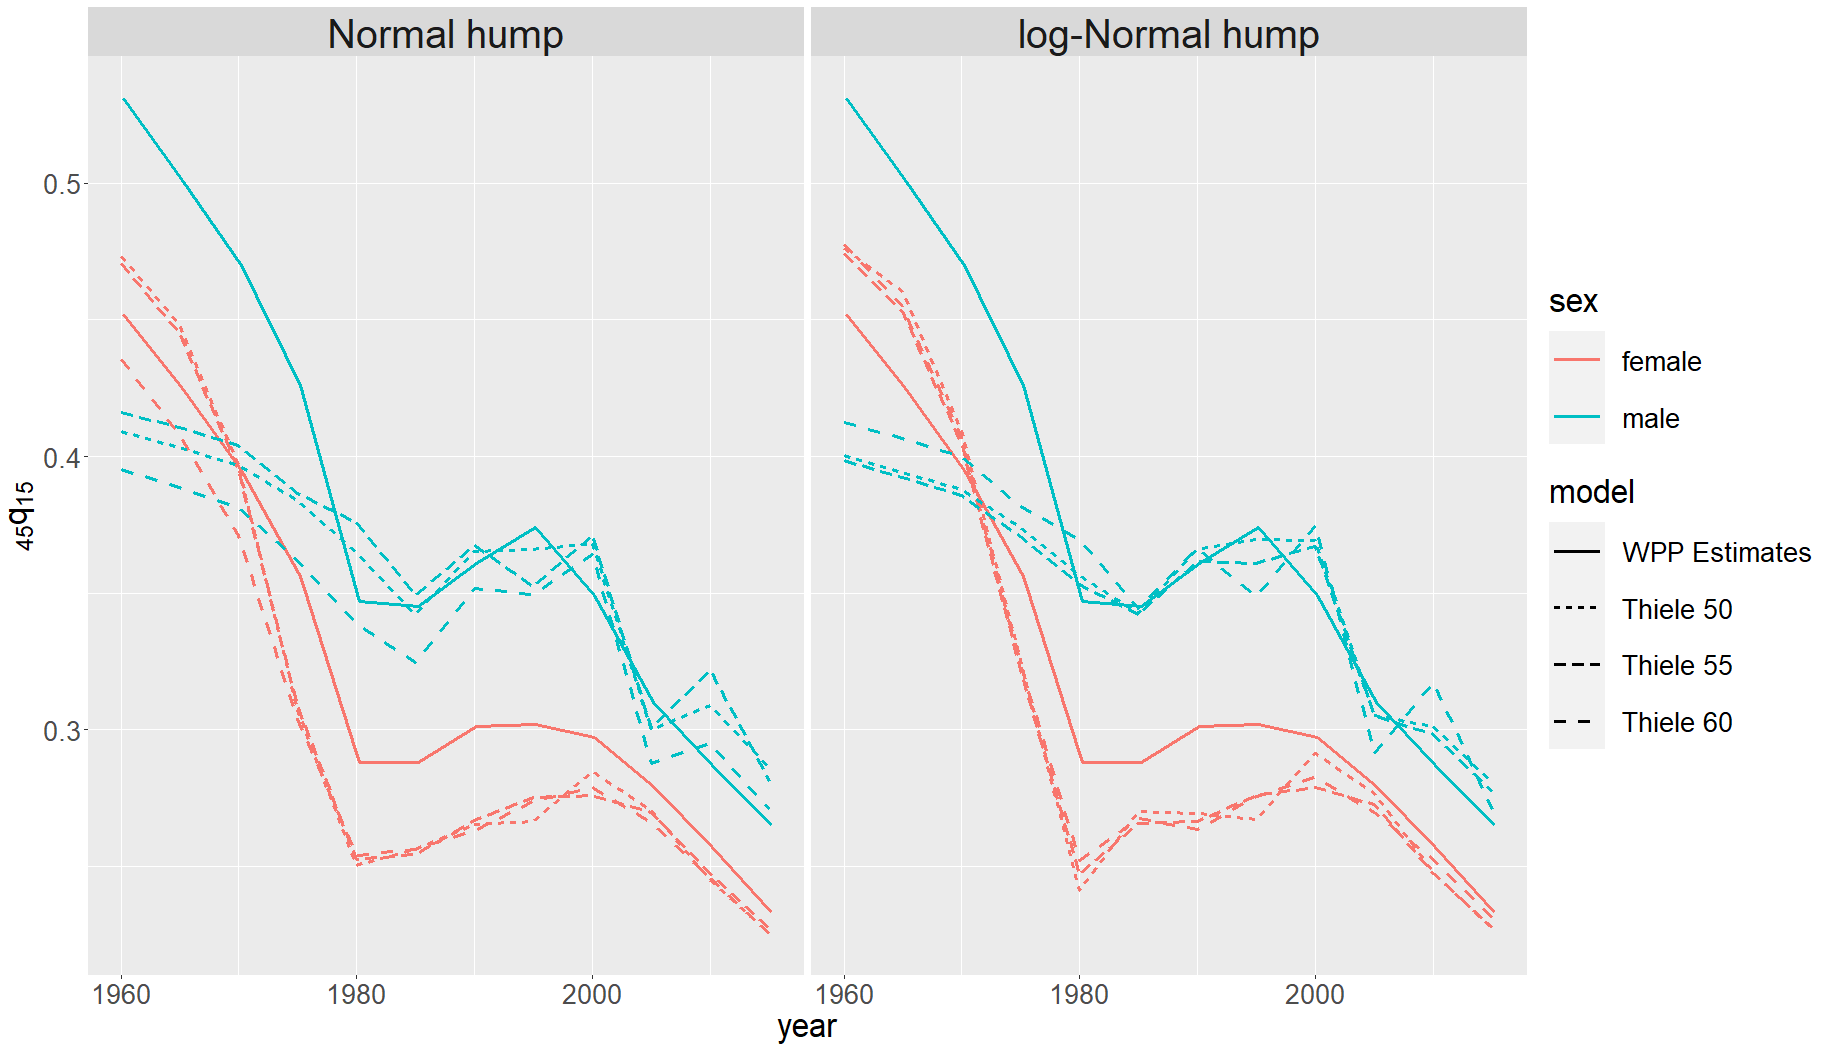
\includegraphics[width = \linewidth]{q4515.png}
\end{figure}
\begin{figure}[H]
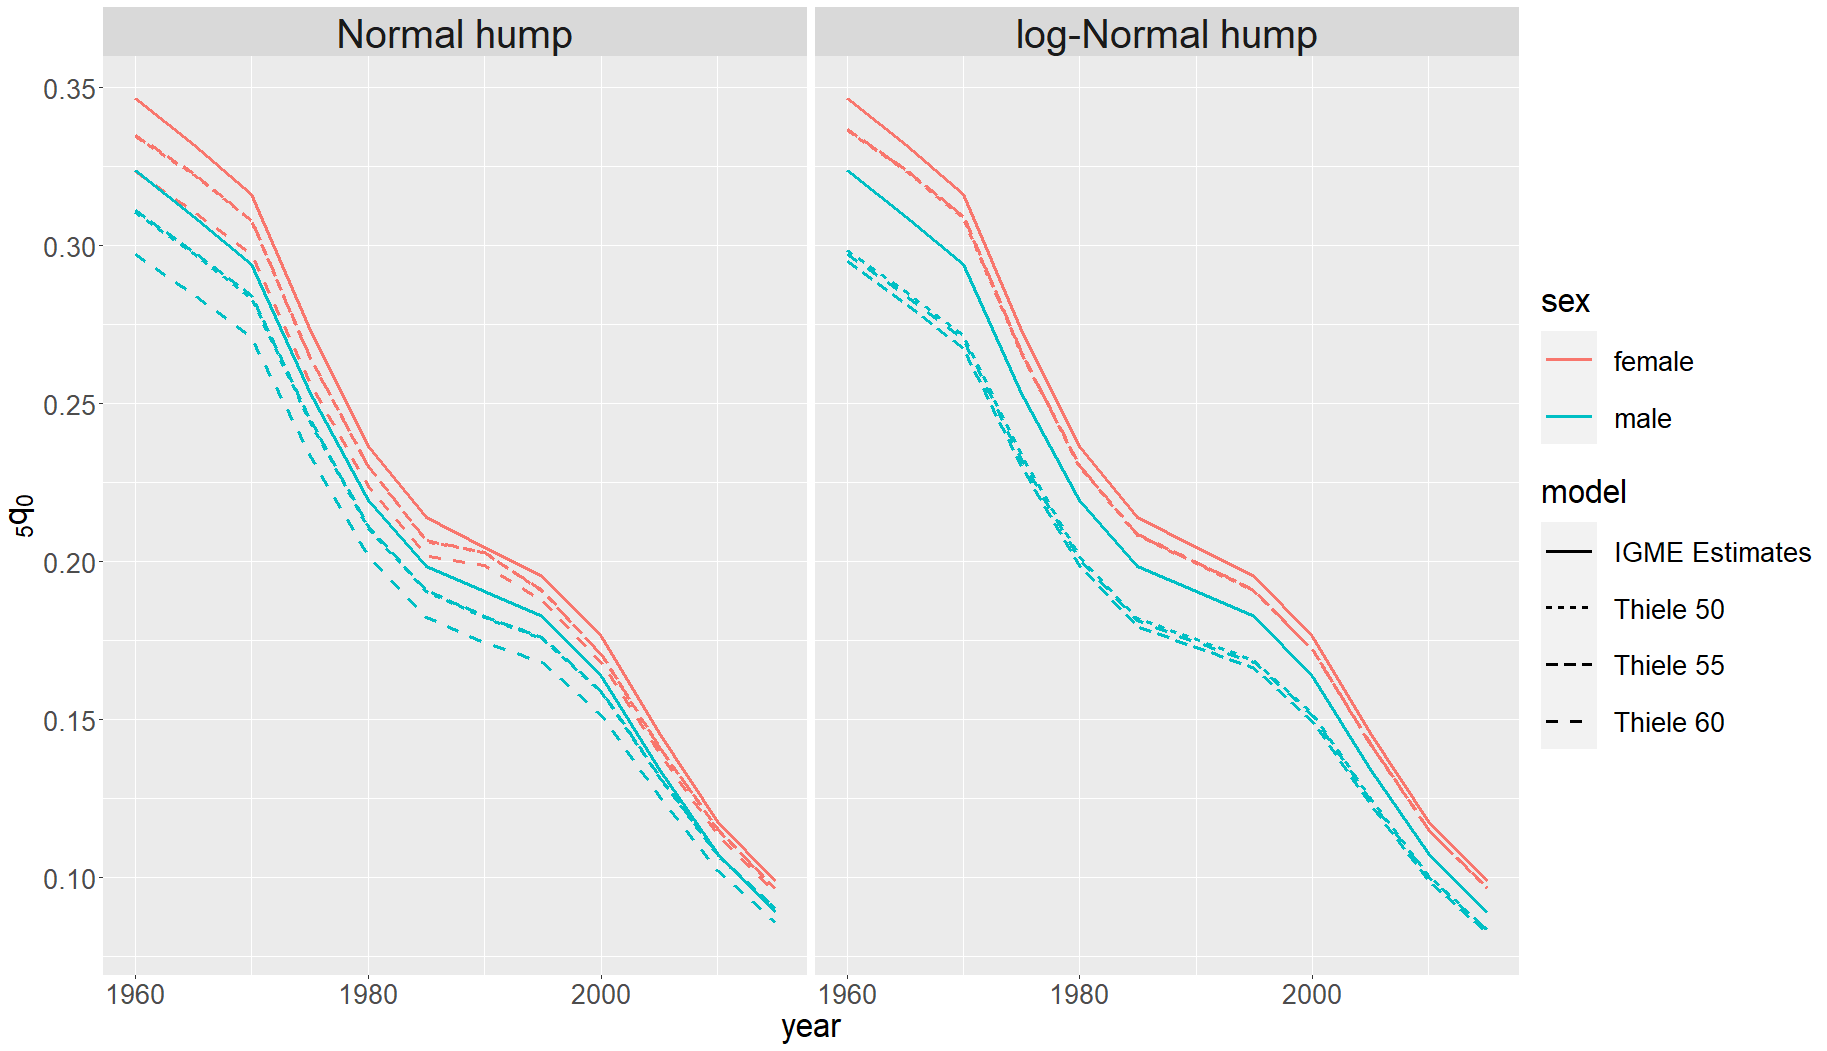
\includegraphics[width = \linewidth]{q50.png}
\end{figure}


\newpage
\begin{figure}[H]
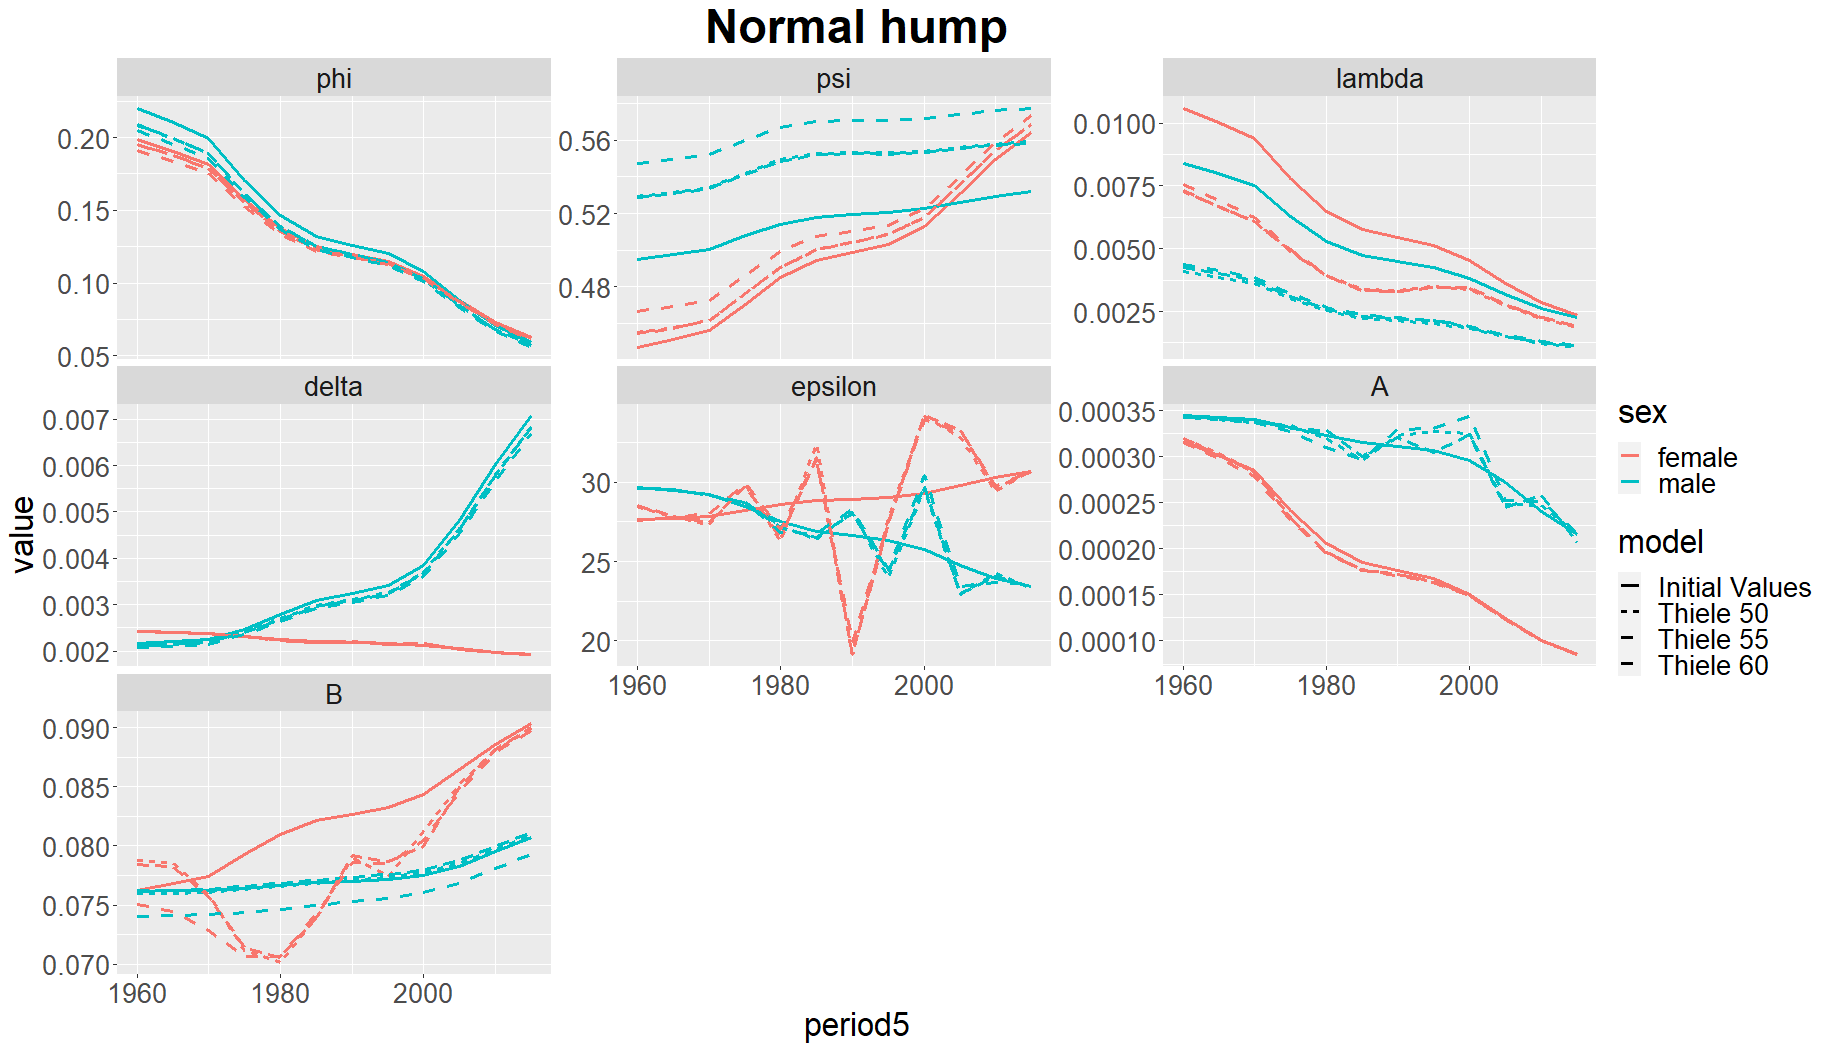
\includegraphics[width = \linewidth]{par normal.png}
\end{figure}
\begin{figure}[H]
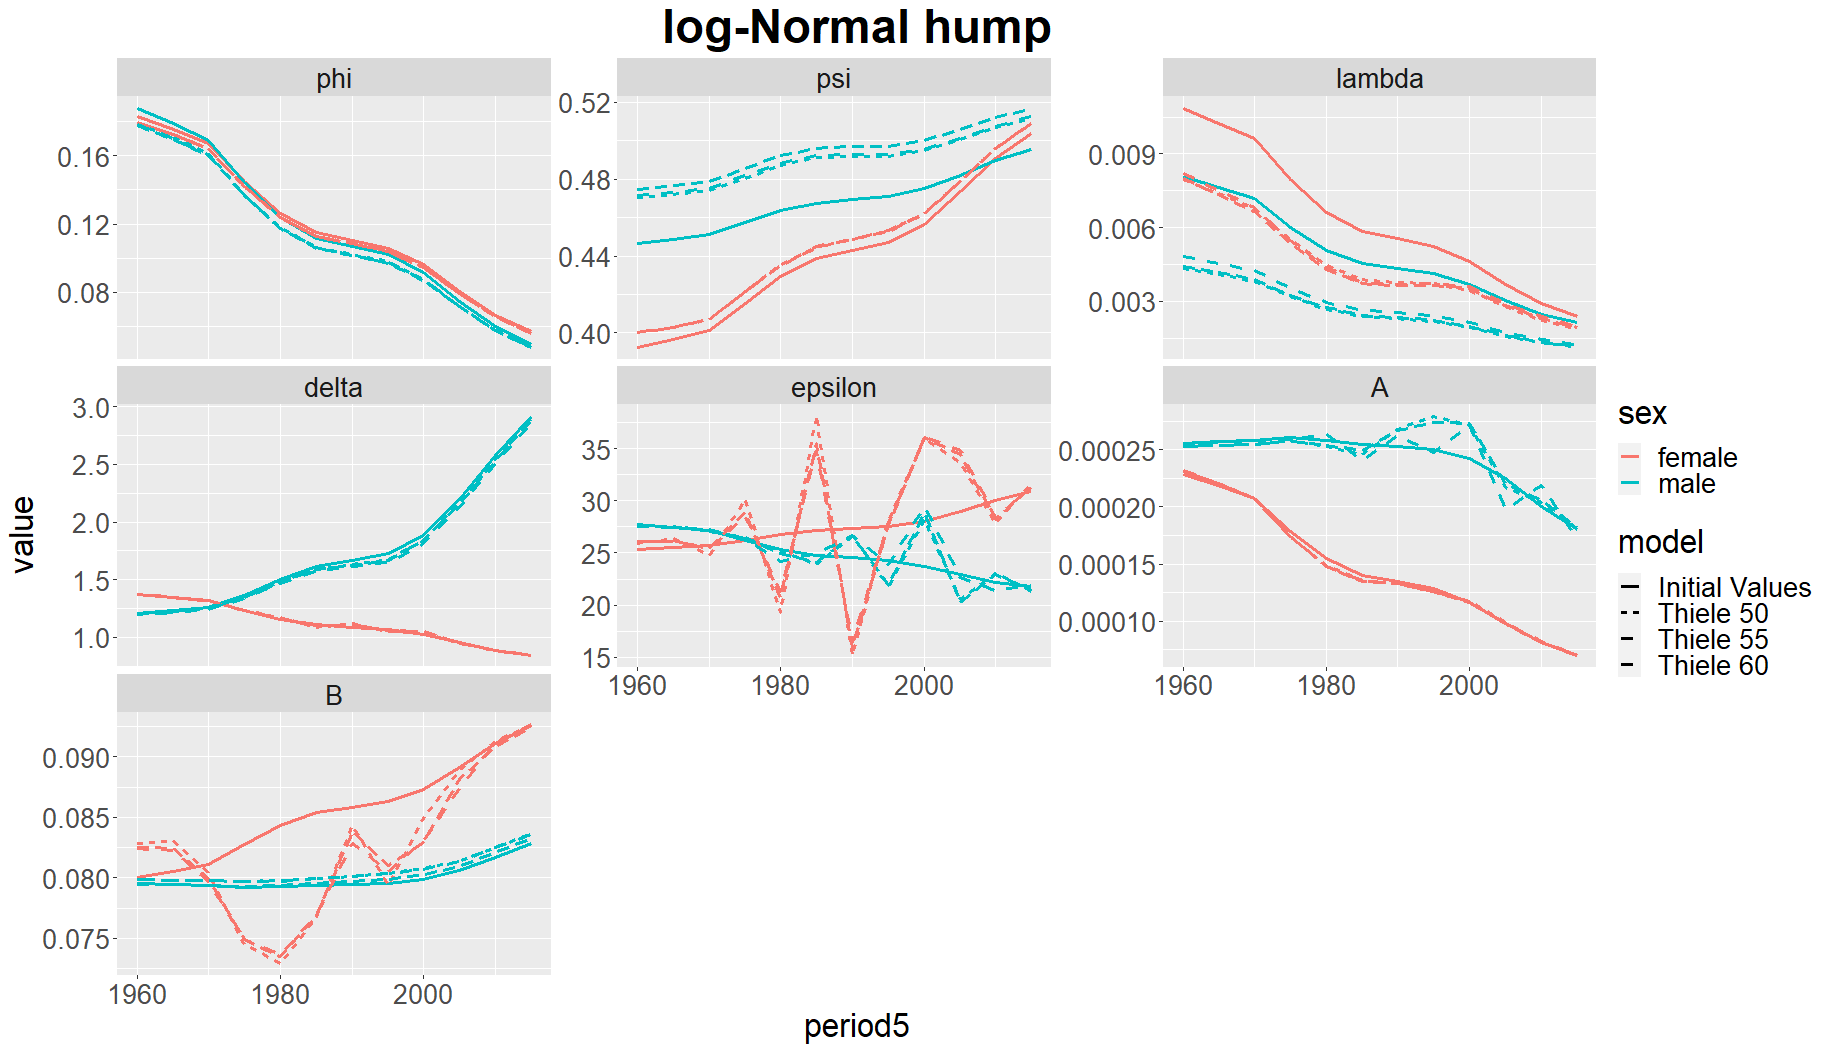
\includegraphics[width = \linewidth]{par log-normal.png}
\end{figure}


\newpage
\begin{figure}[H]
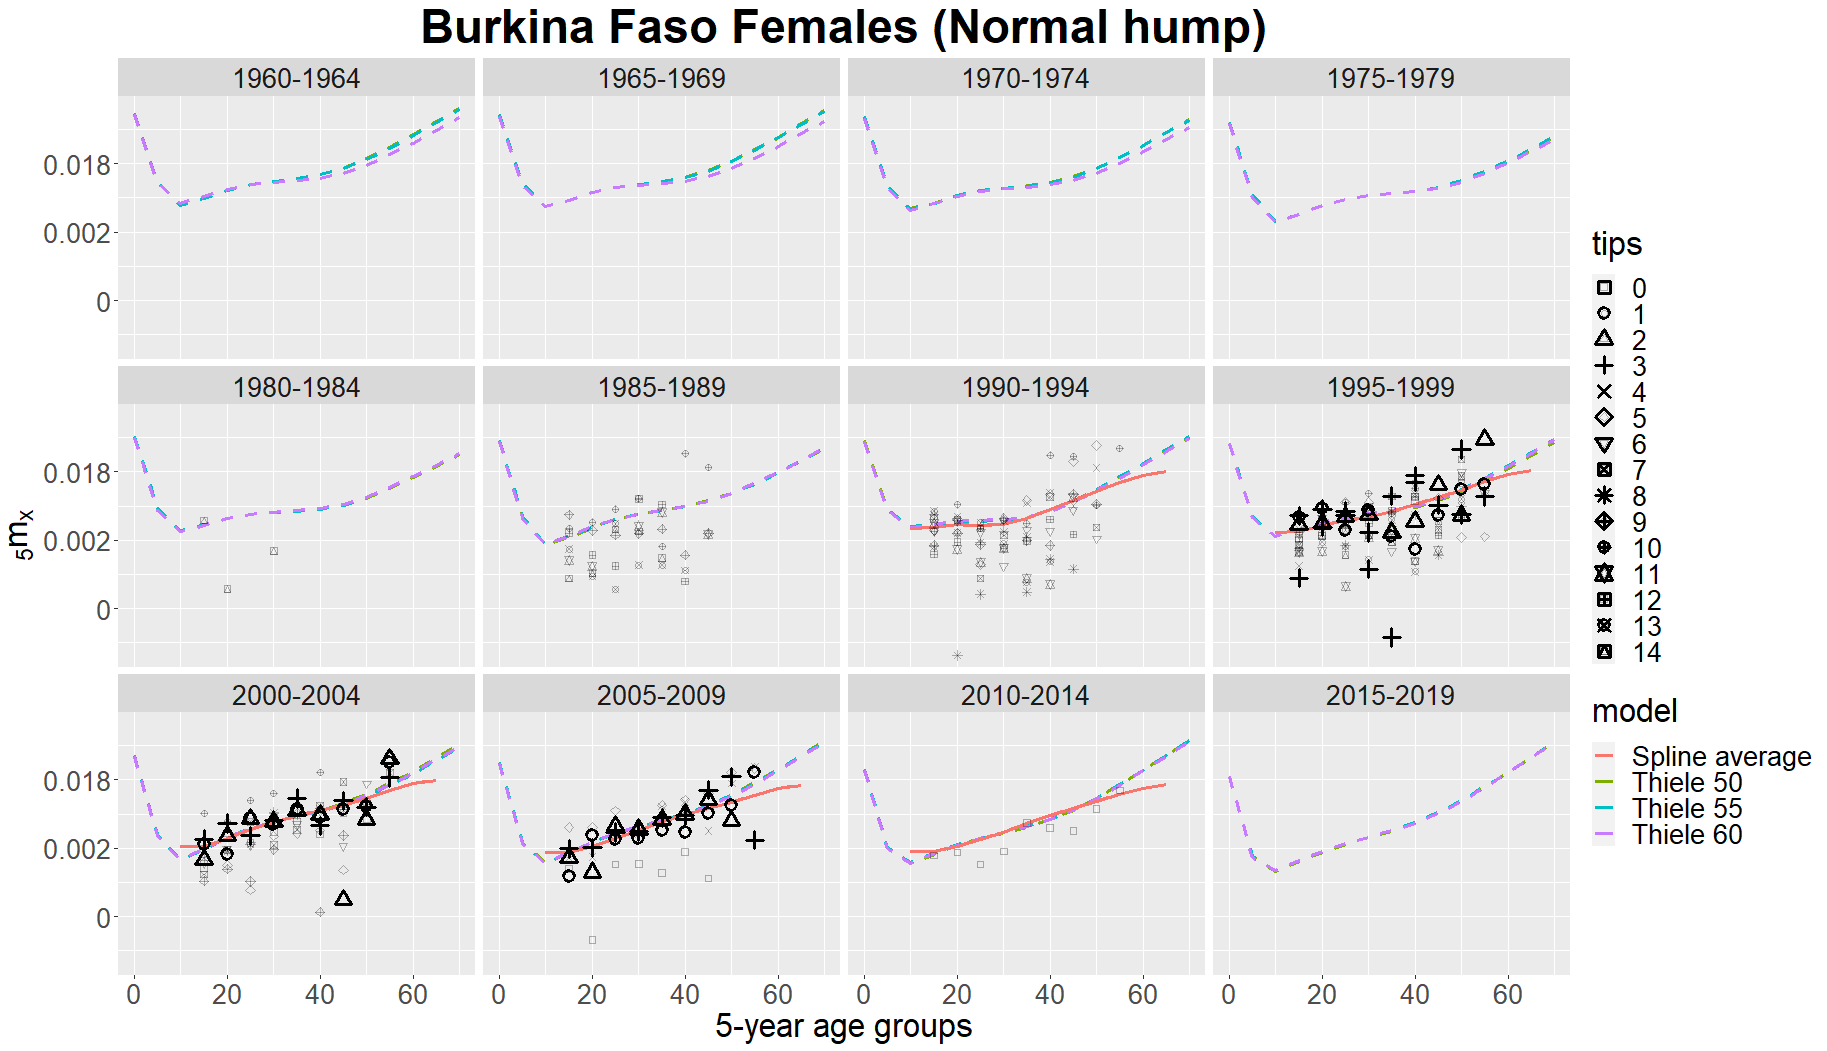
\includegraphics[width = \linewidth]{dhs females normal.png}
\end{figure}
\begin{figure}[H]
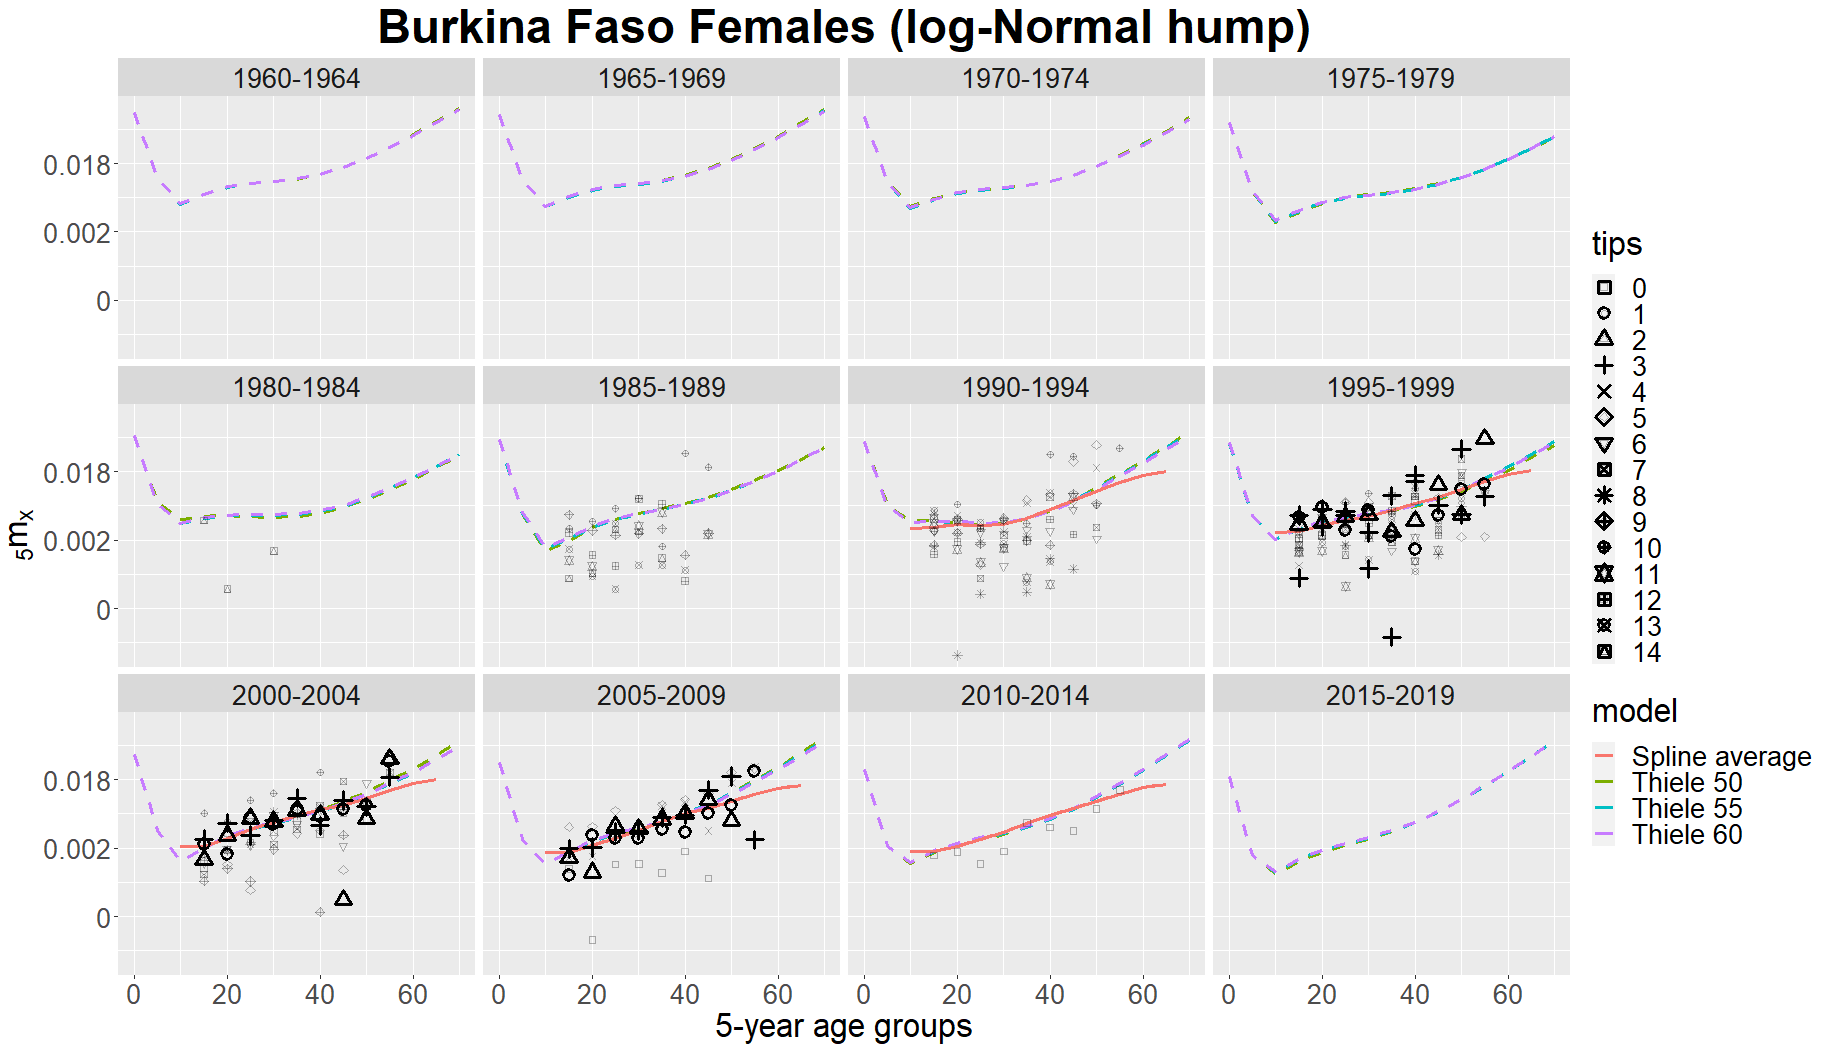
\includegraphics[width = \linewidth]{dhs females log-normal.png}
\end{figure}

\newpage
\begin{figure}[H]
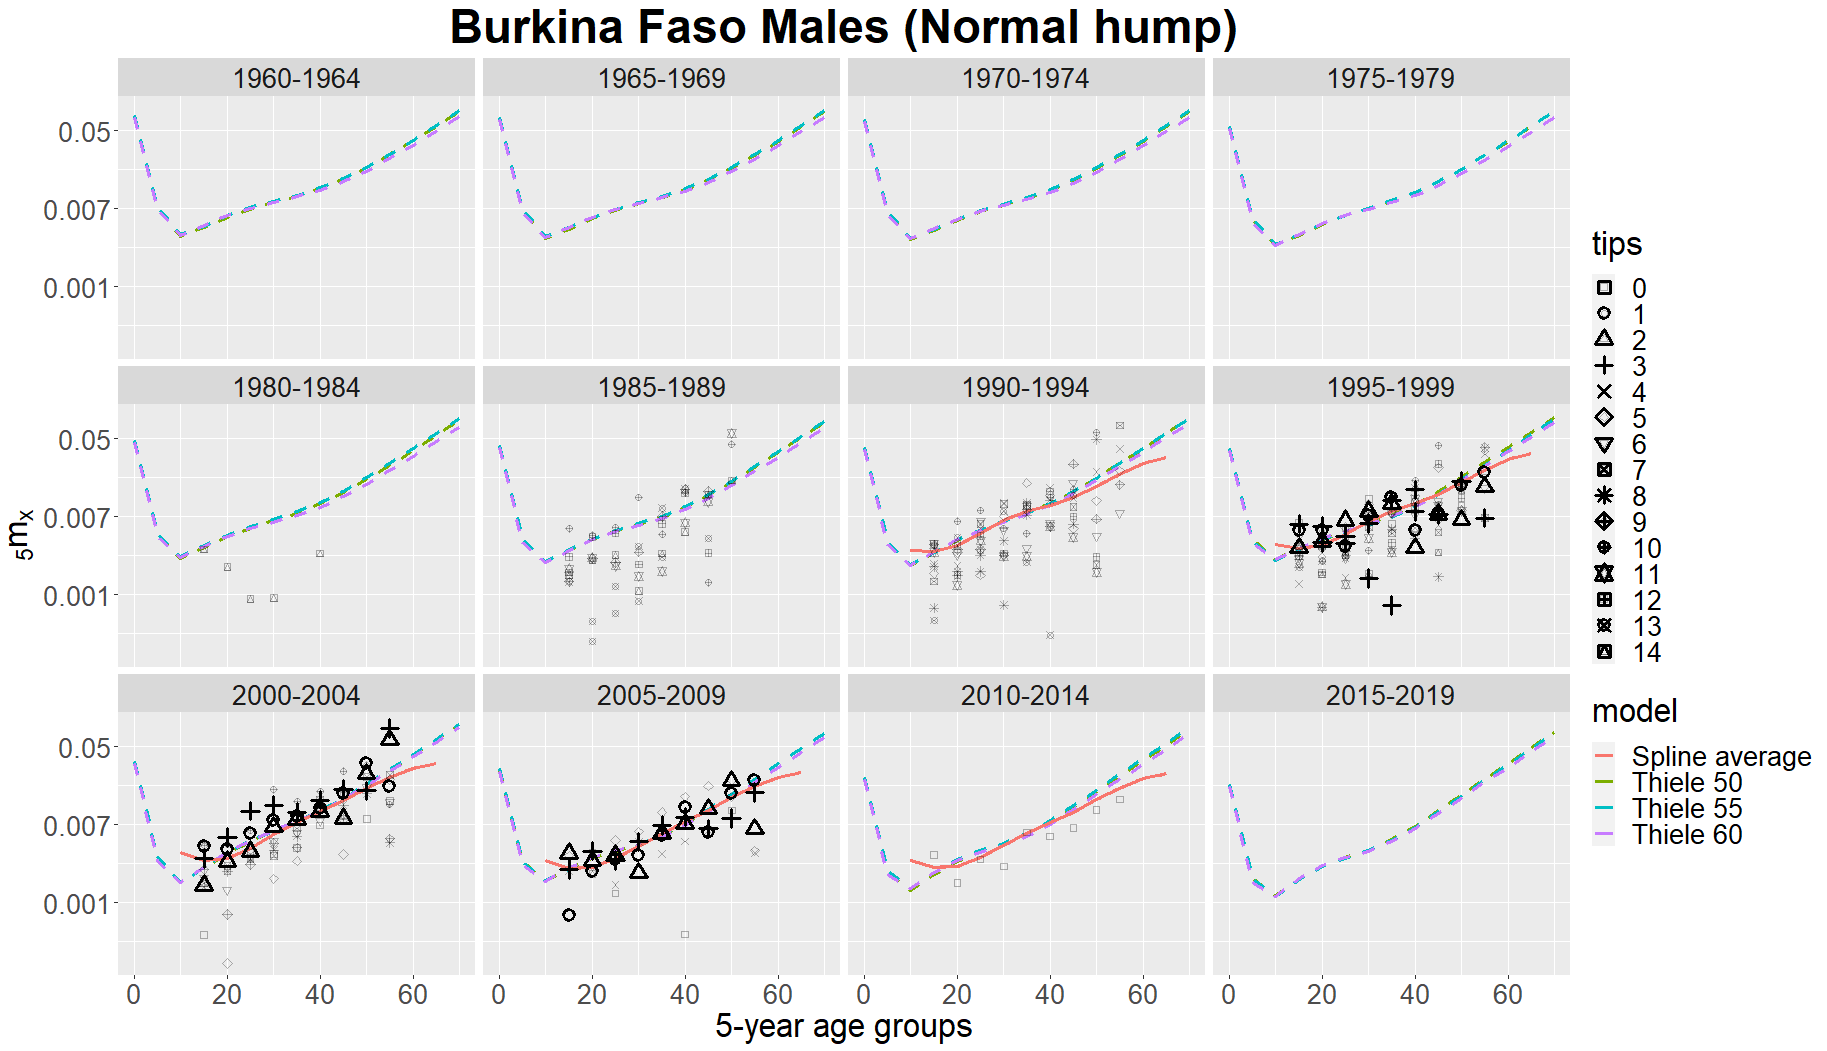
\includegraphics[width = \linewidth]{dhs males normal.png}
\end{figure}
\begin{figure}[H]
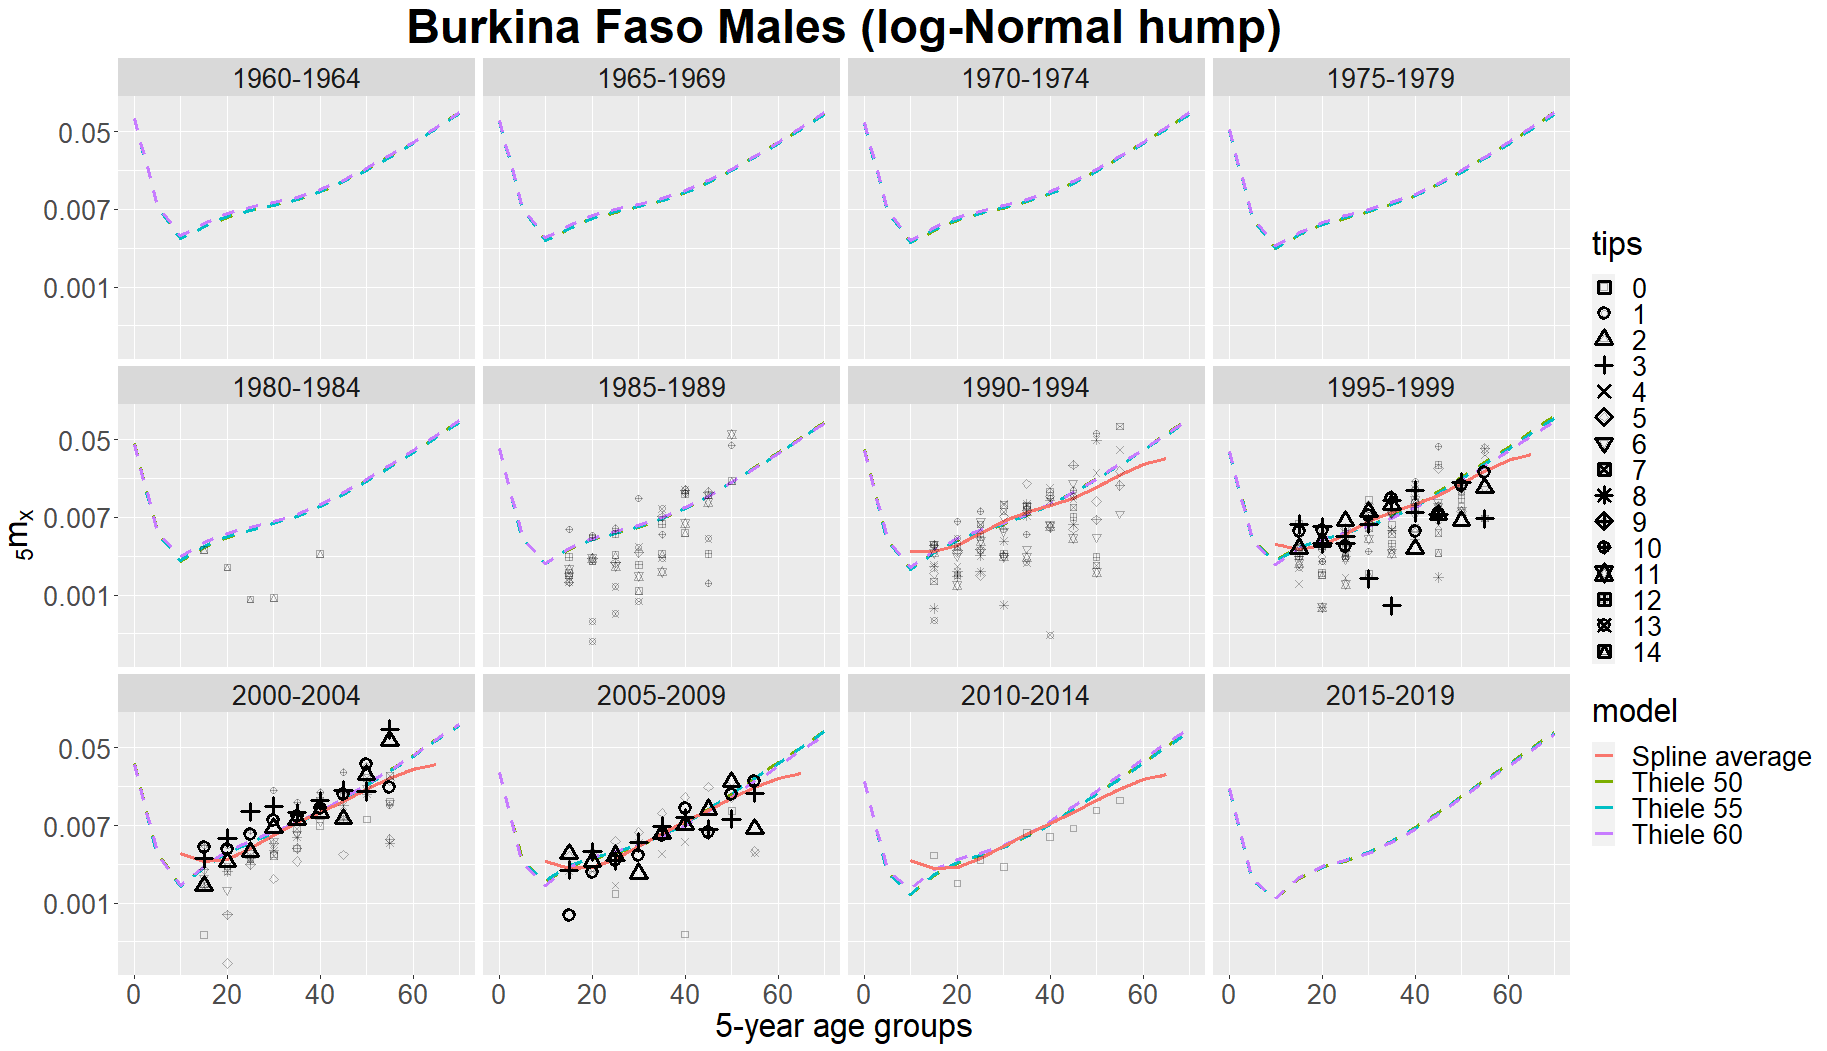
\includegraphics[width = \linewidth]{dhs males log-normal.png}
\end{figure}


\newpage
\begin{figure}[H]
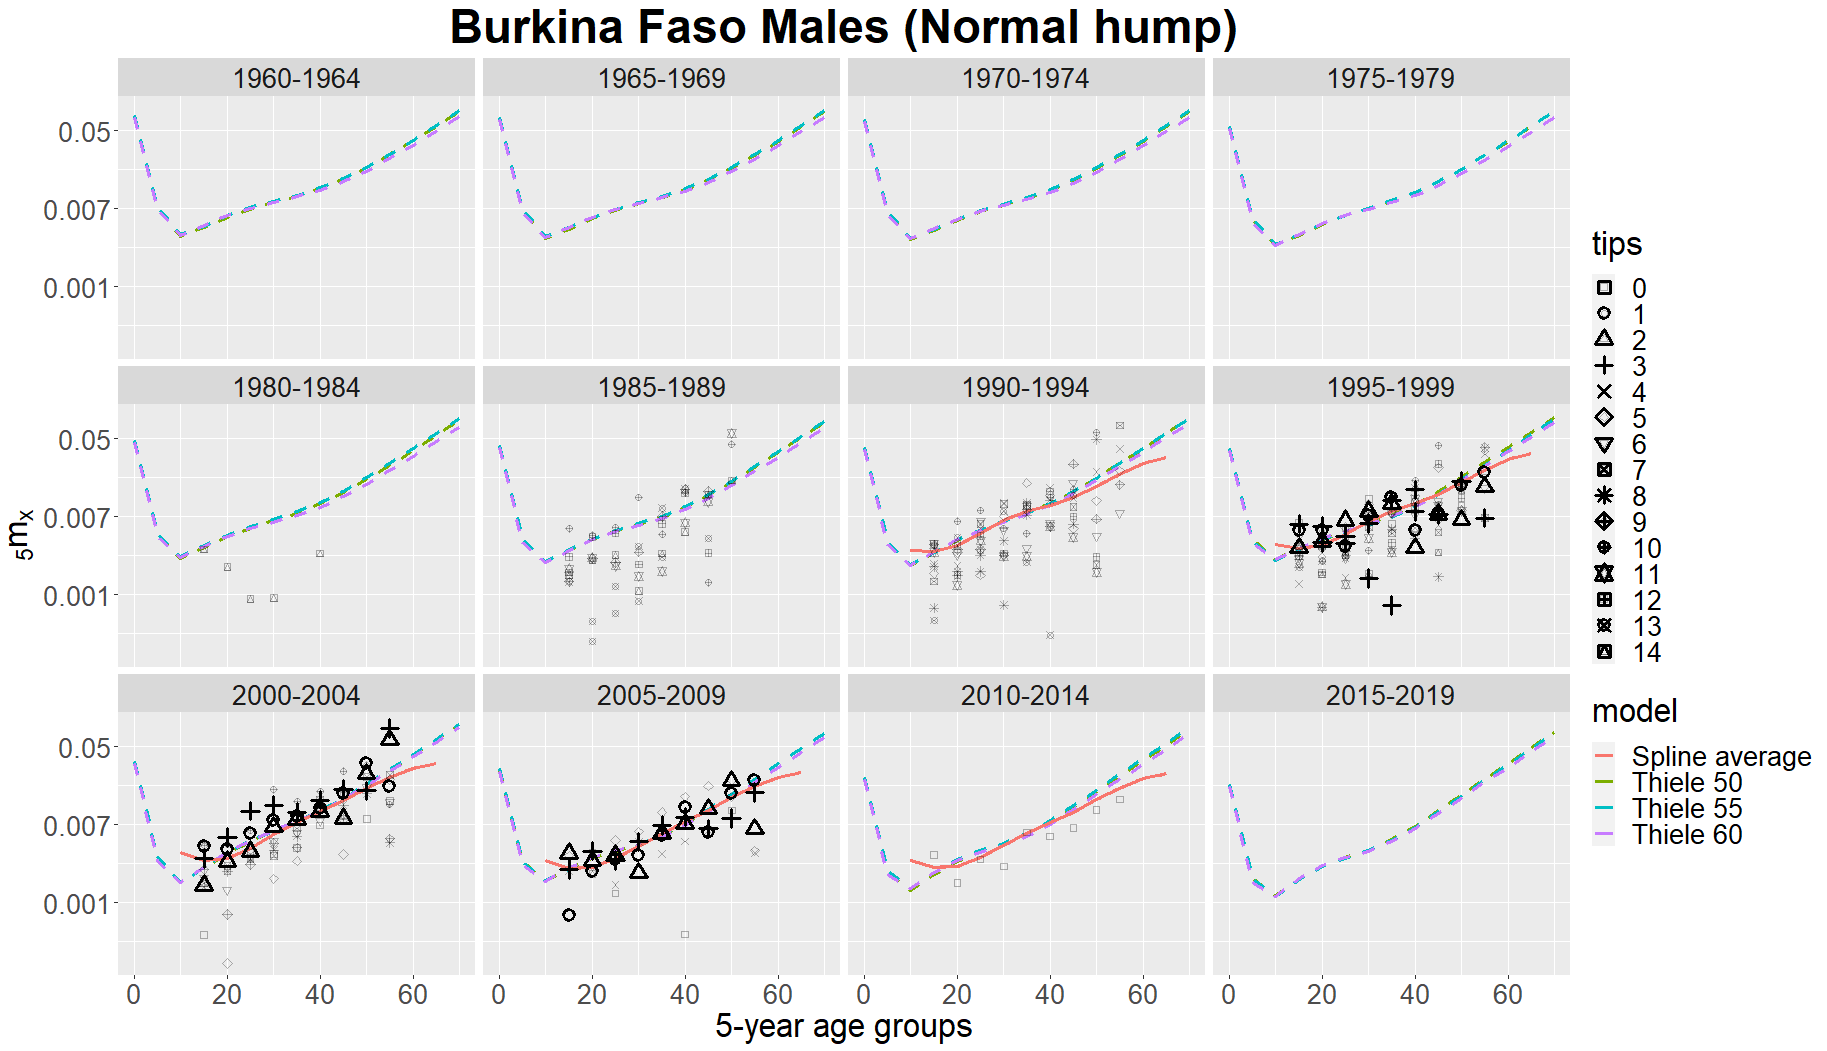
\includegraphics[width = \linewidth]{dhs males normal.png}
\end{figure}
\begin{figure}[H]
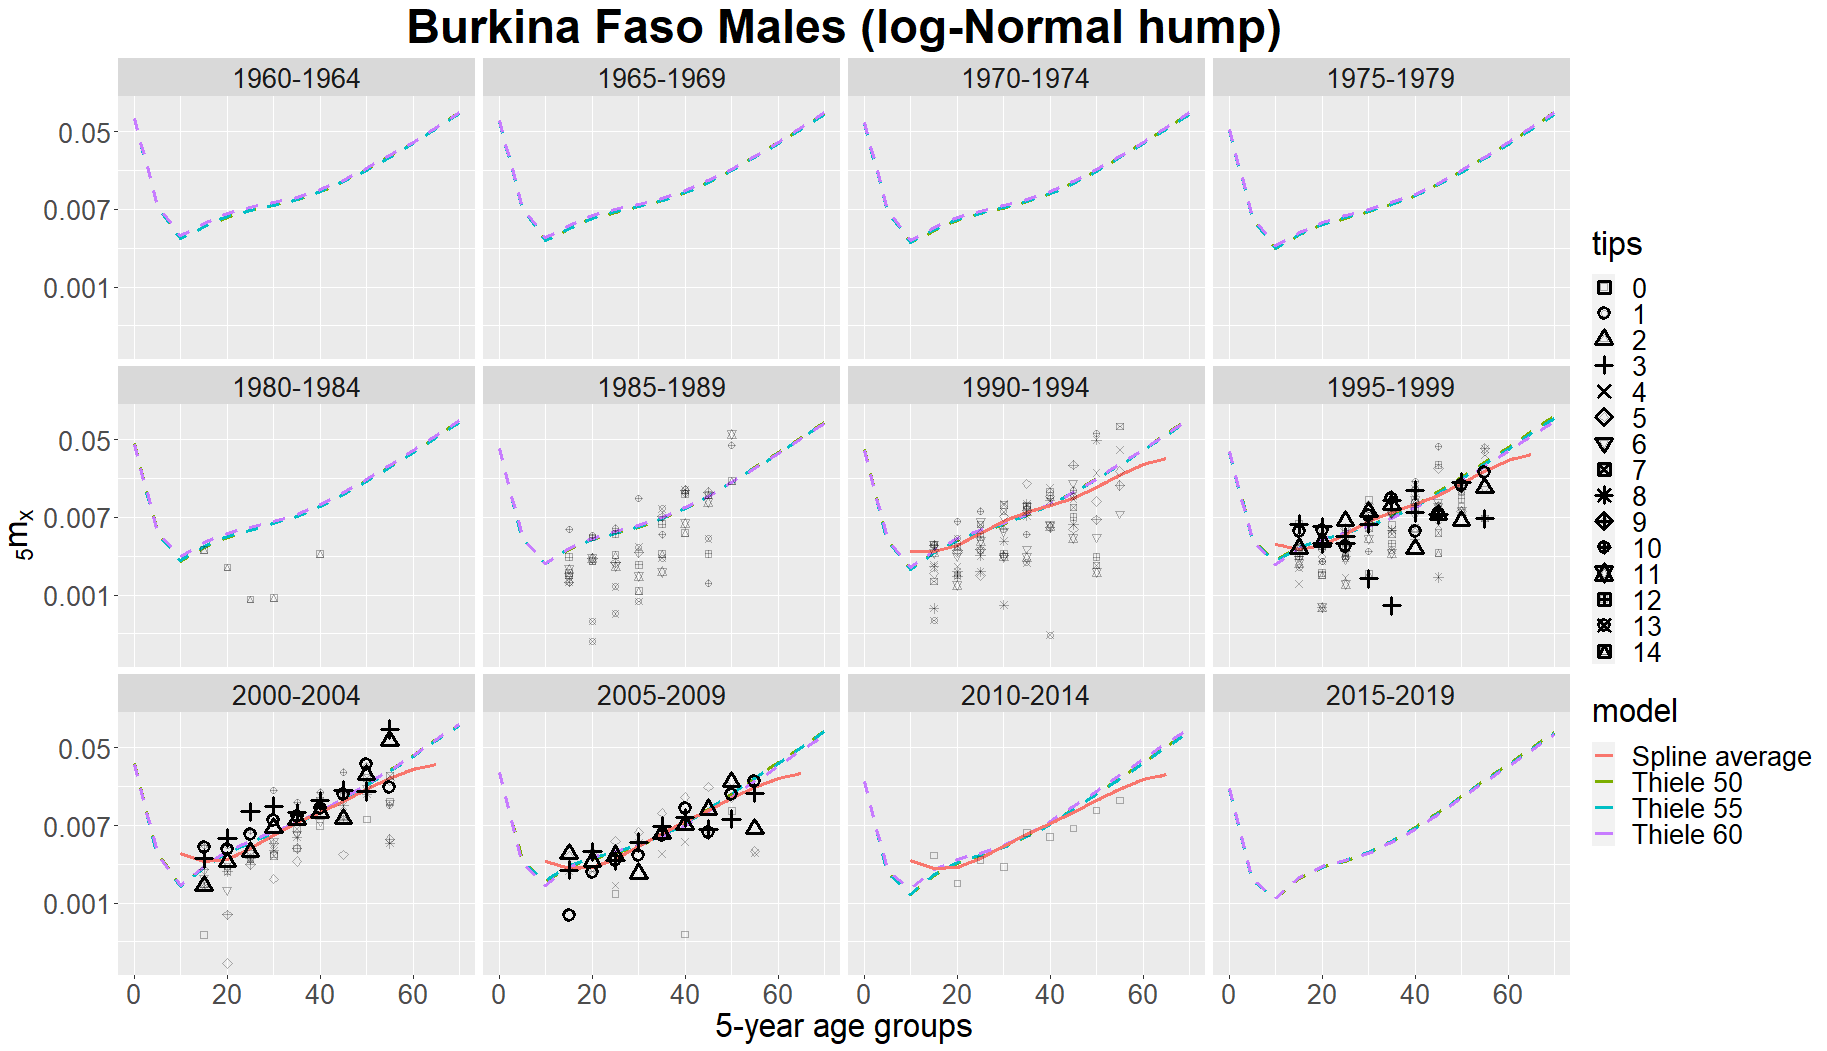
\includegraphics[width = \linewidth]{dhs males log-normal.png}
\end{figure}

\newpage
\begin{figure}[H]
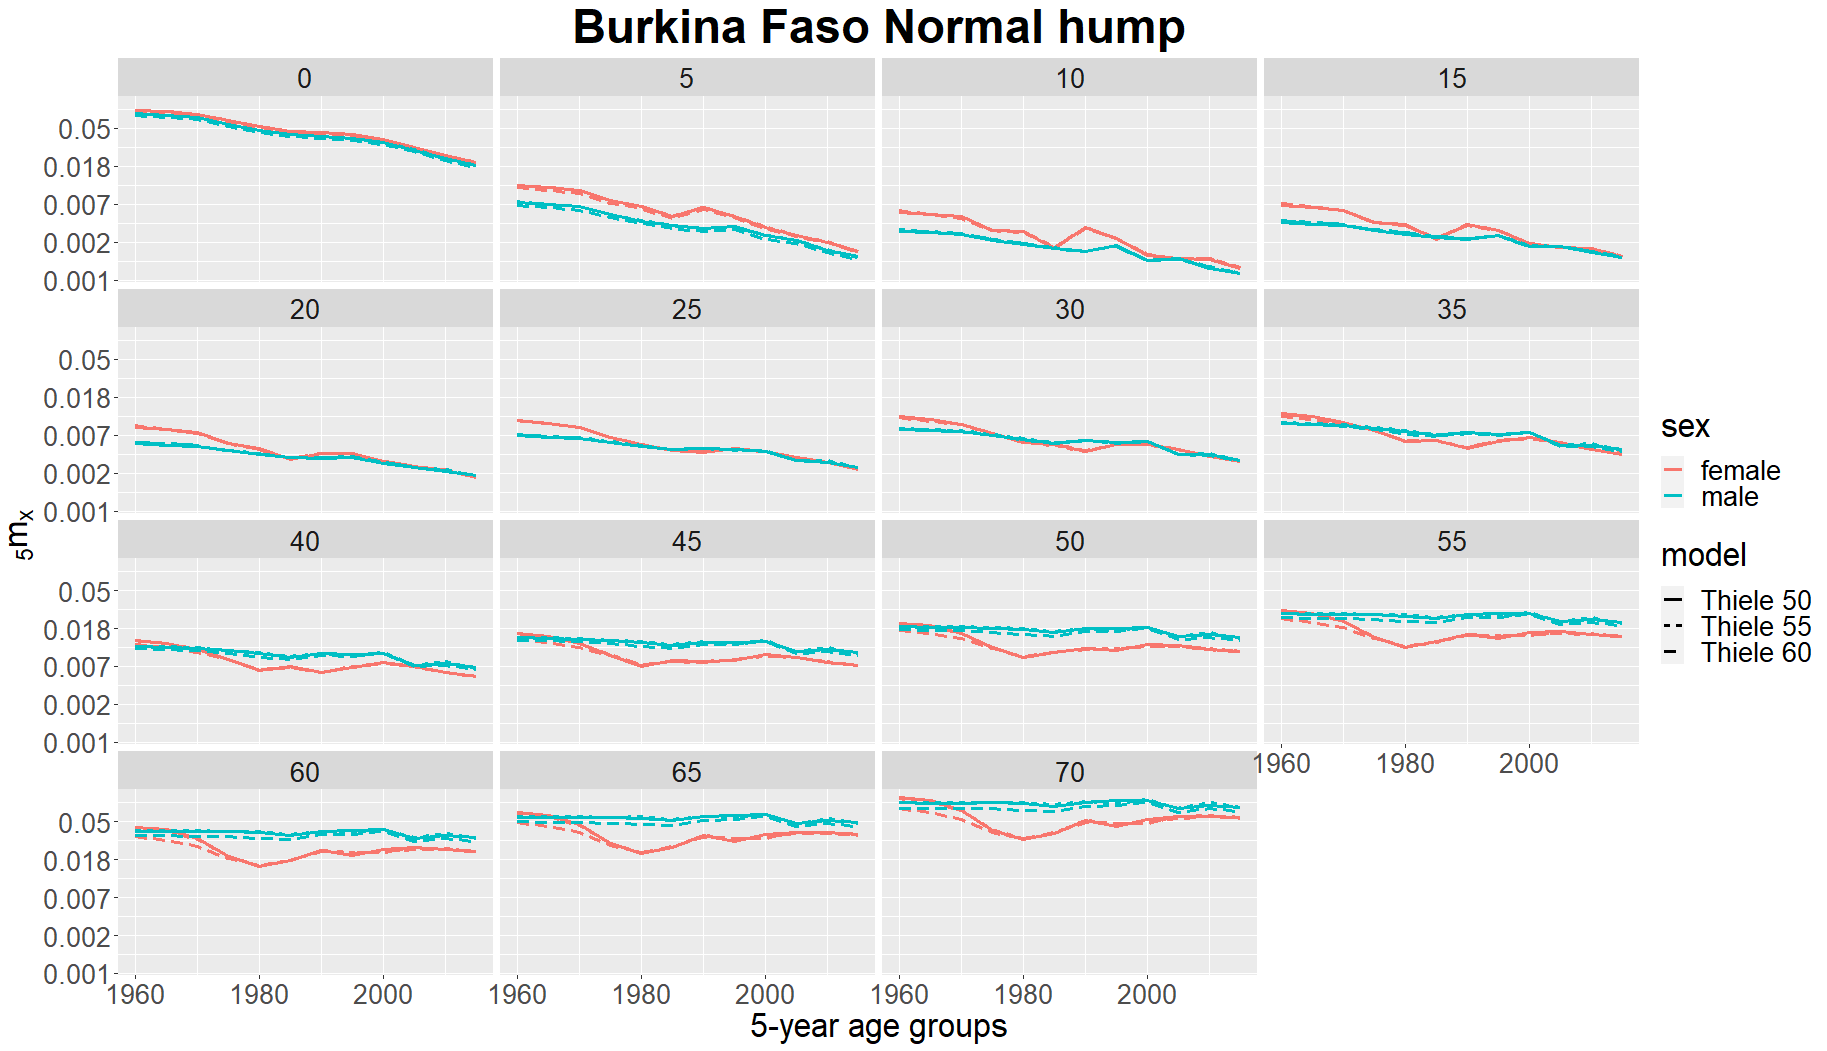
\includegraphics[width = \linewidth]{age mx normal.png}
\end{figure}
\begin{figure}[H]
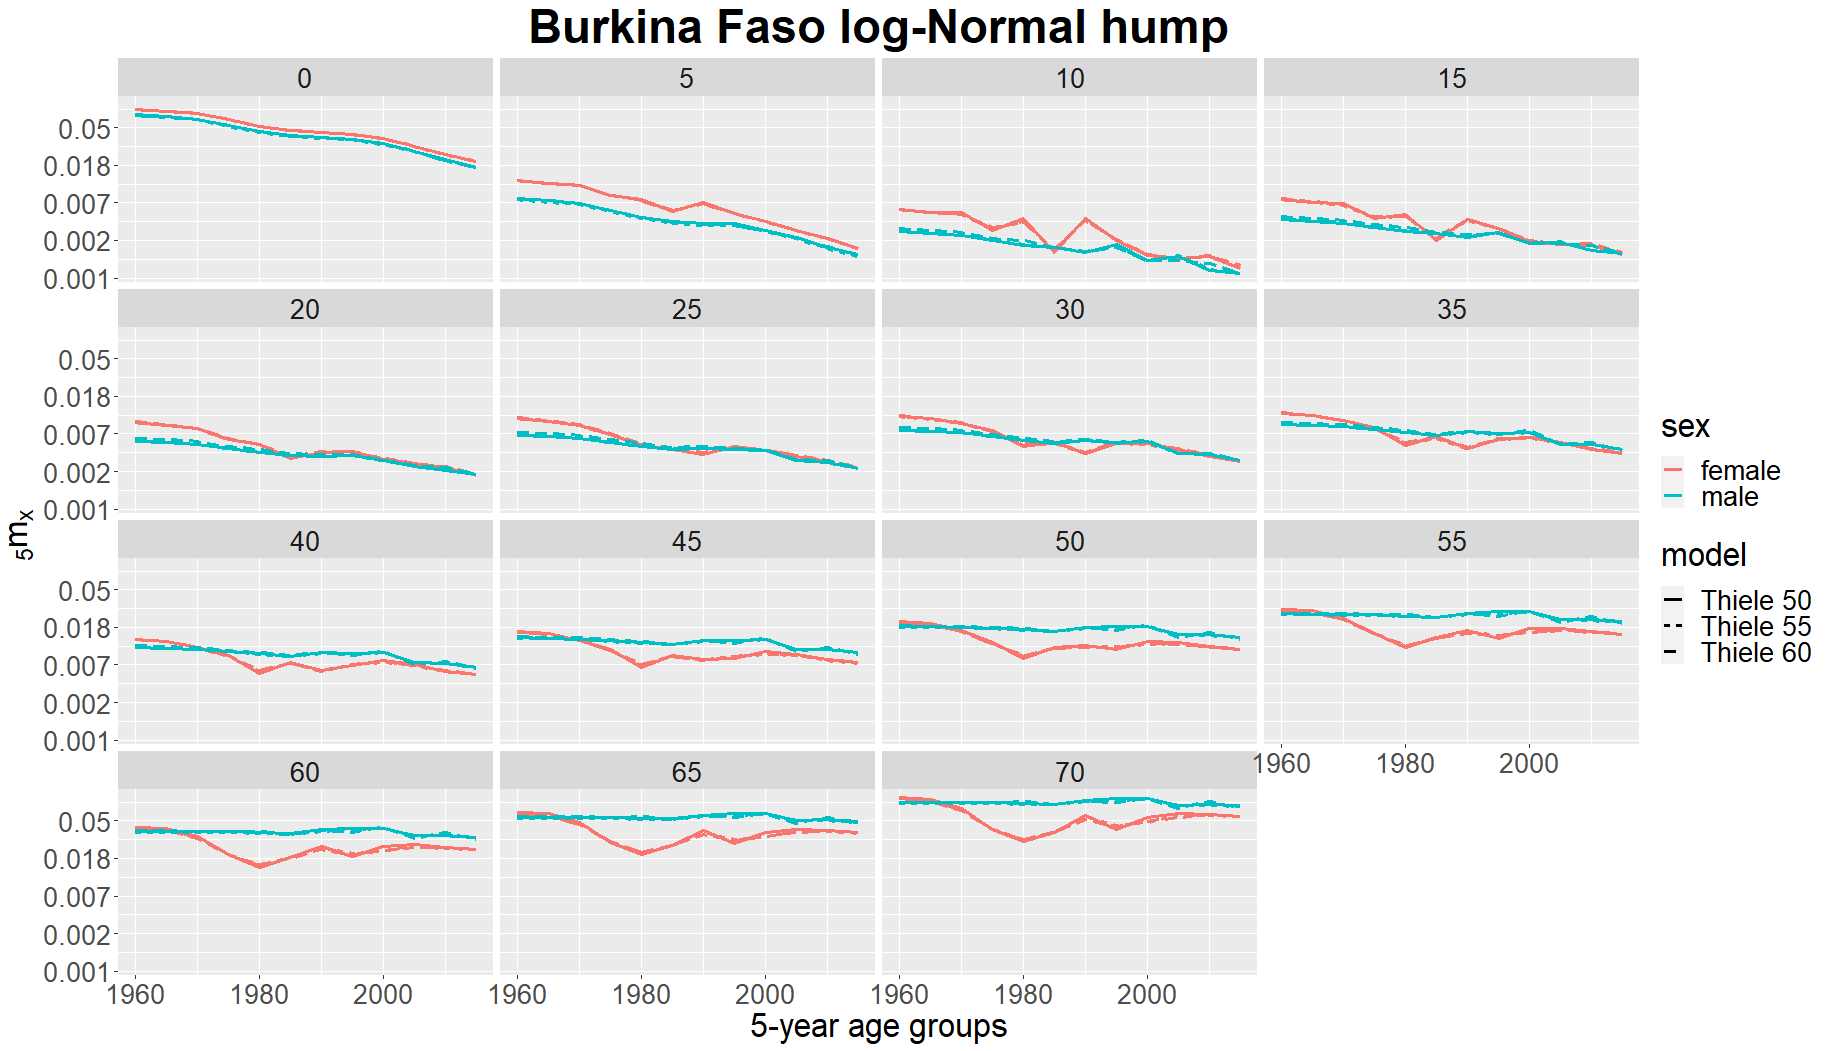
\includegraphics[width = \linewidth]{age mx log-normal.png}
\end{figure}


\newpage
\begin{figure}[H]
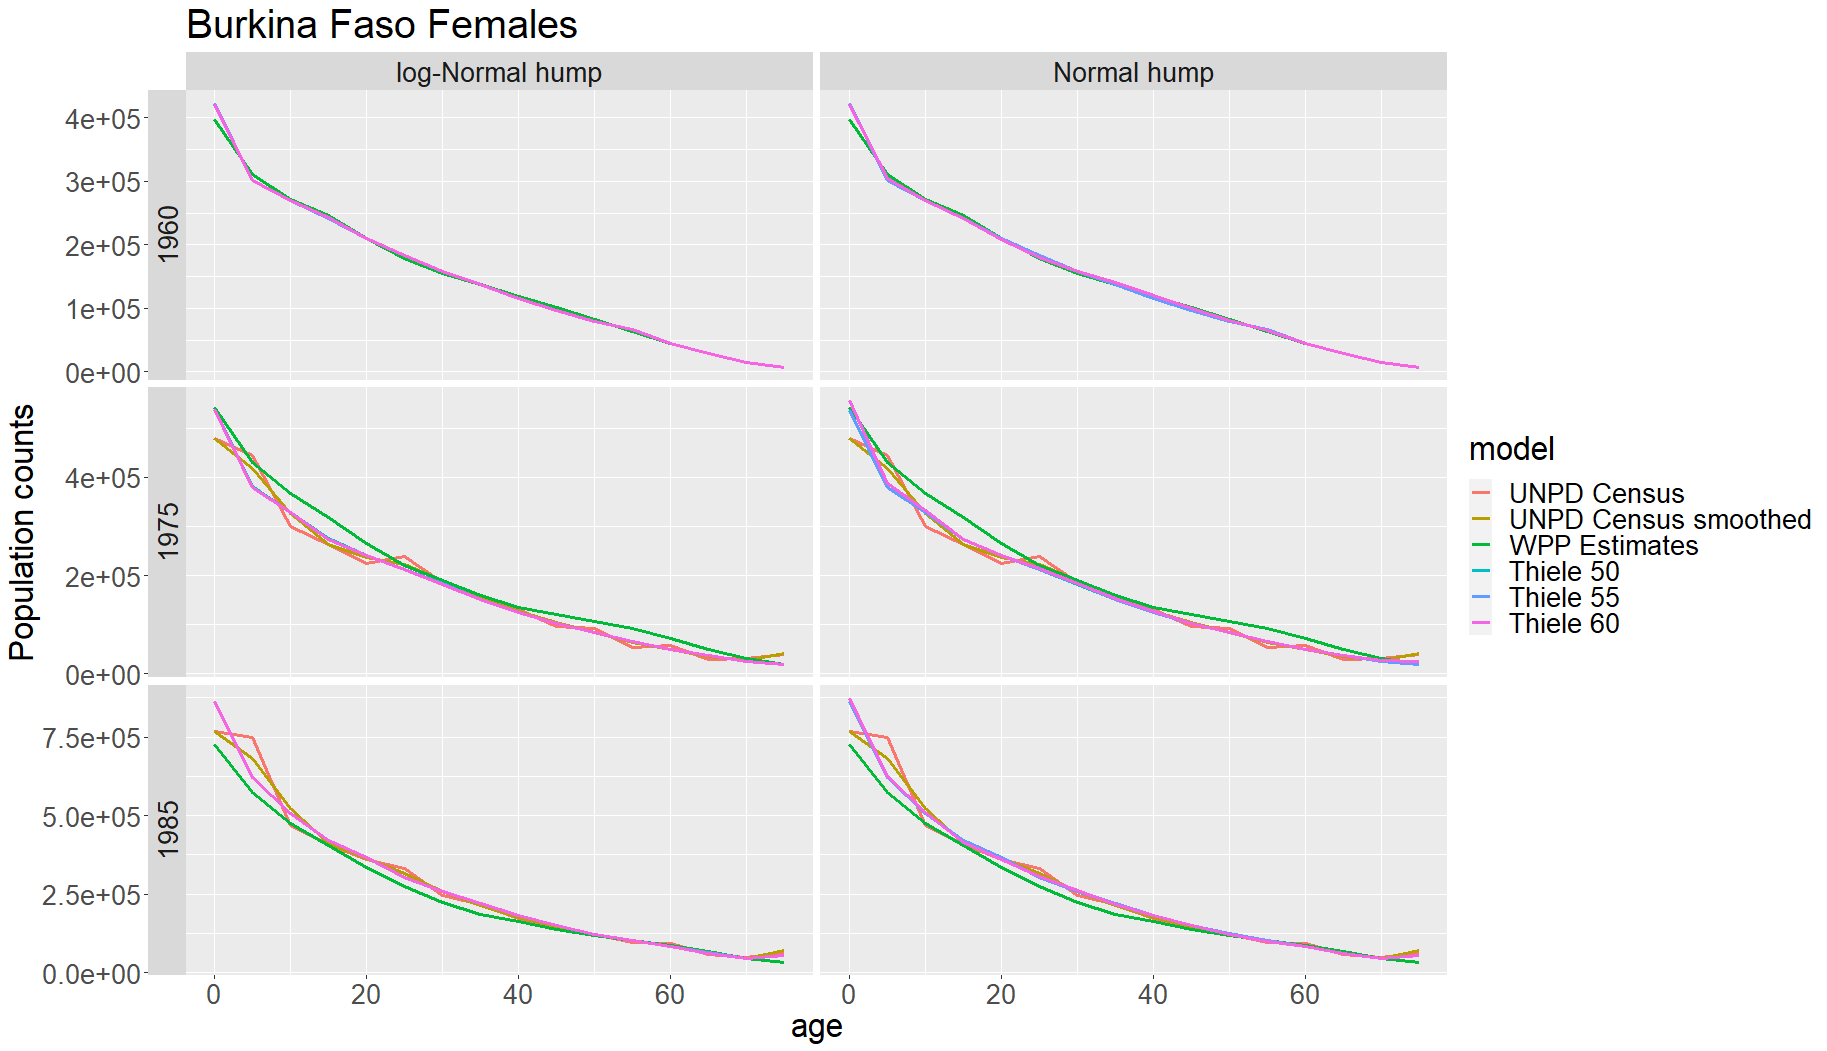
\includegraphics[width = \linewidth]{pop females.png}
\end{figure}
\begin{figure}[H]
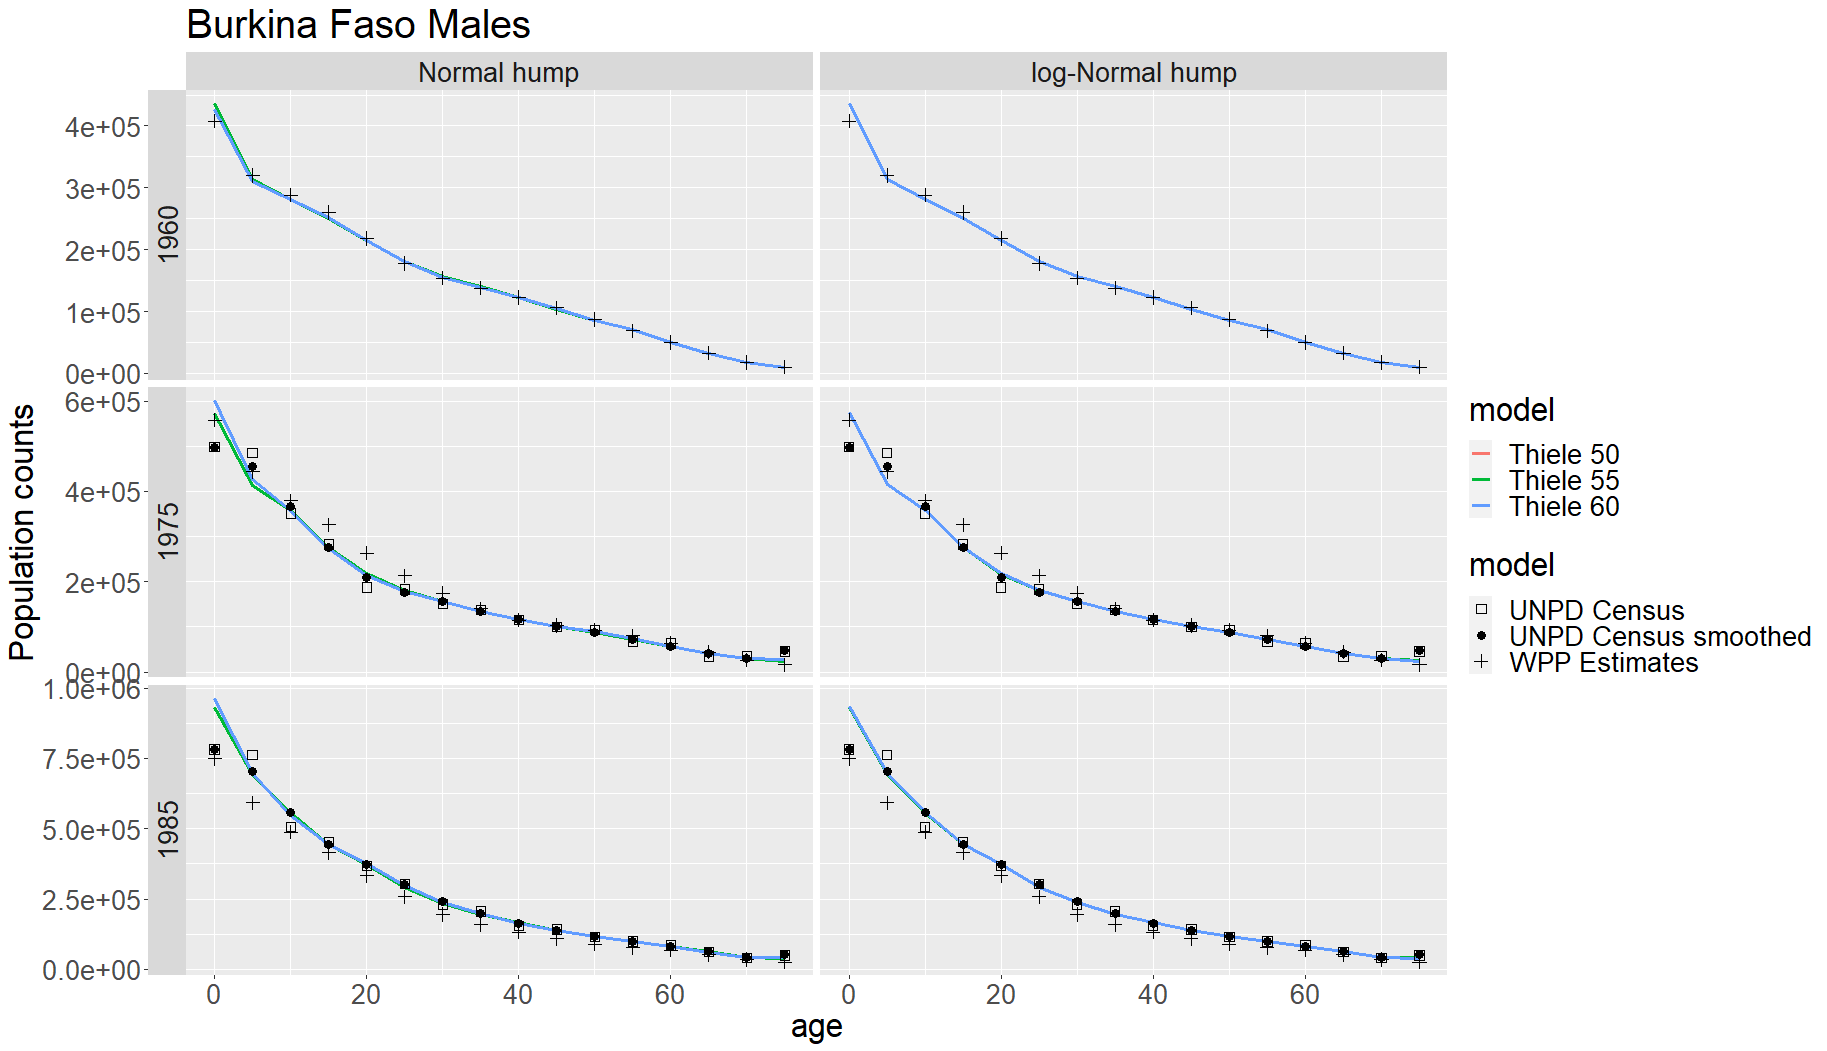
\includegraphics[width = \linewidth]{pop males.png}
\end{figure}


\newpage
\begin{figure}[H]
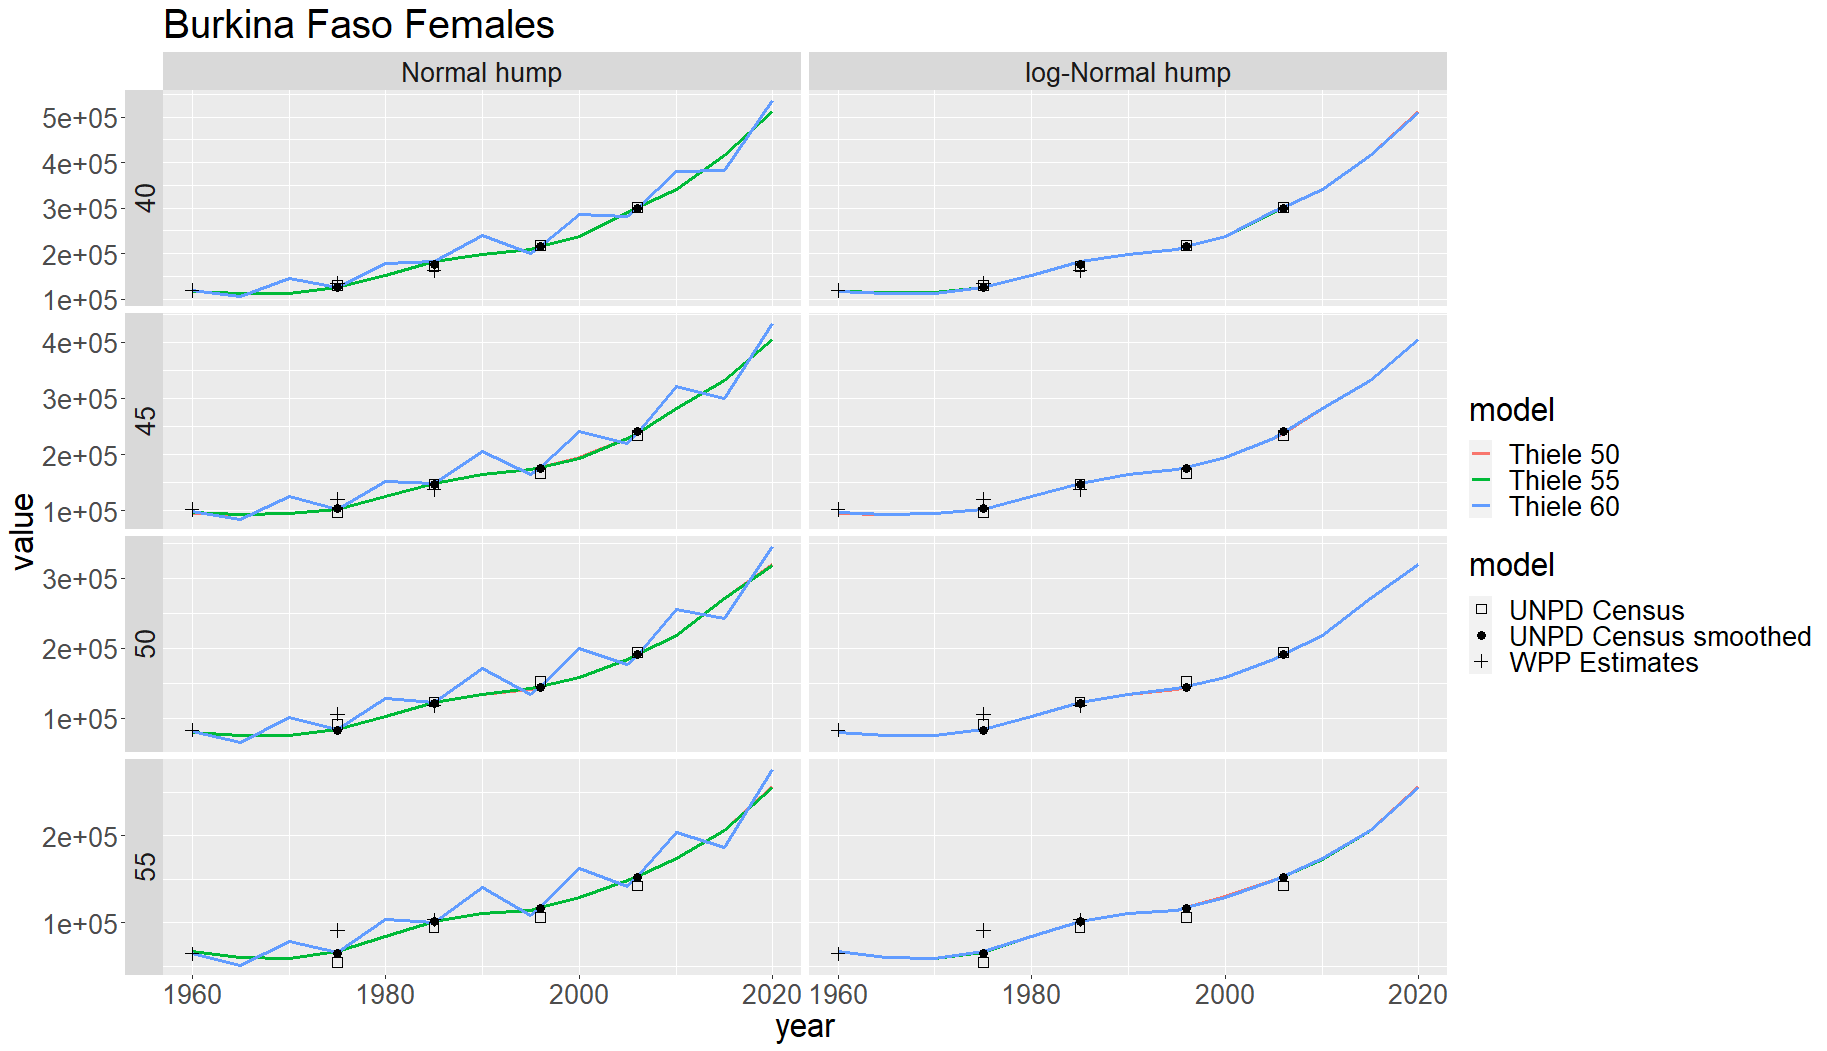
\includegraphics[width = \linewidth]{age pop females.png}
\end{figure}
\begin{figure}[H]
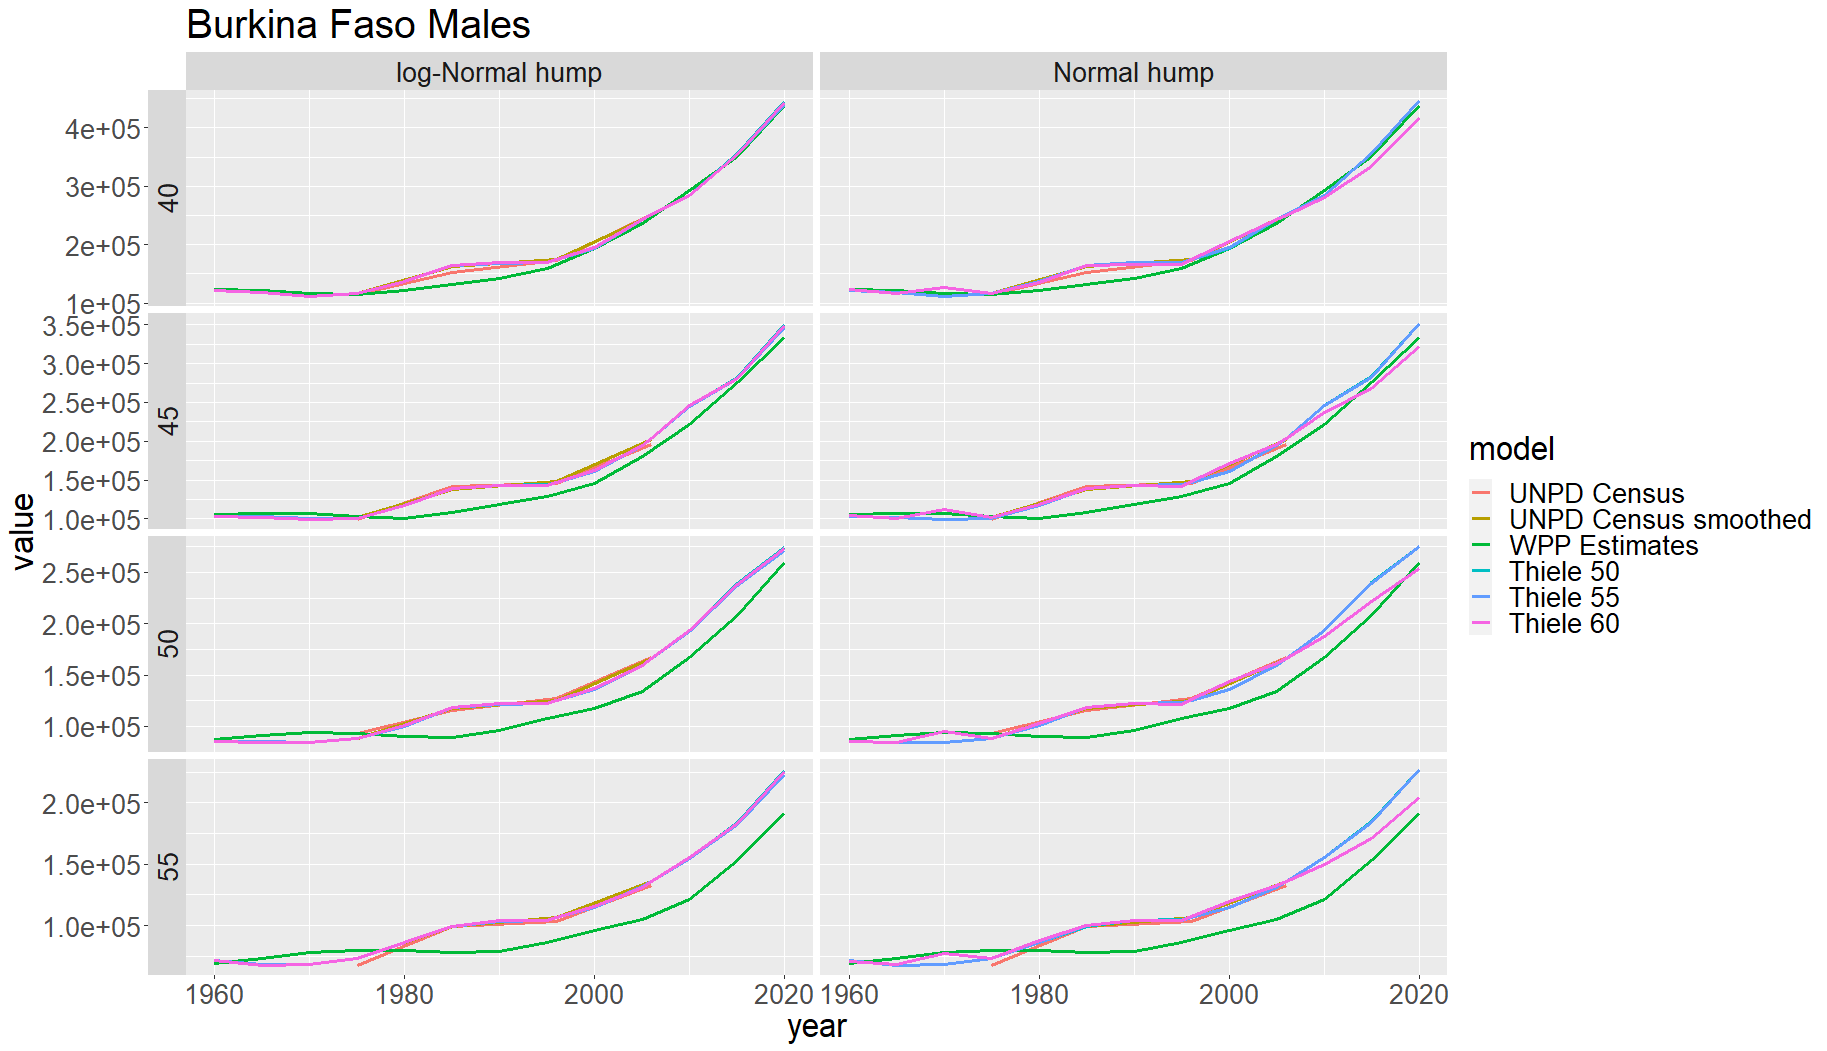
\includegraphics[width = \linewidth]{age pop males.png}
\end{figure}

\newpage
\begin{figure}[H]
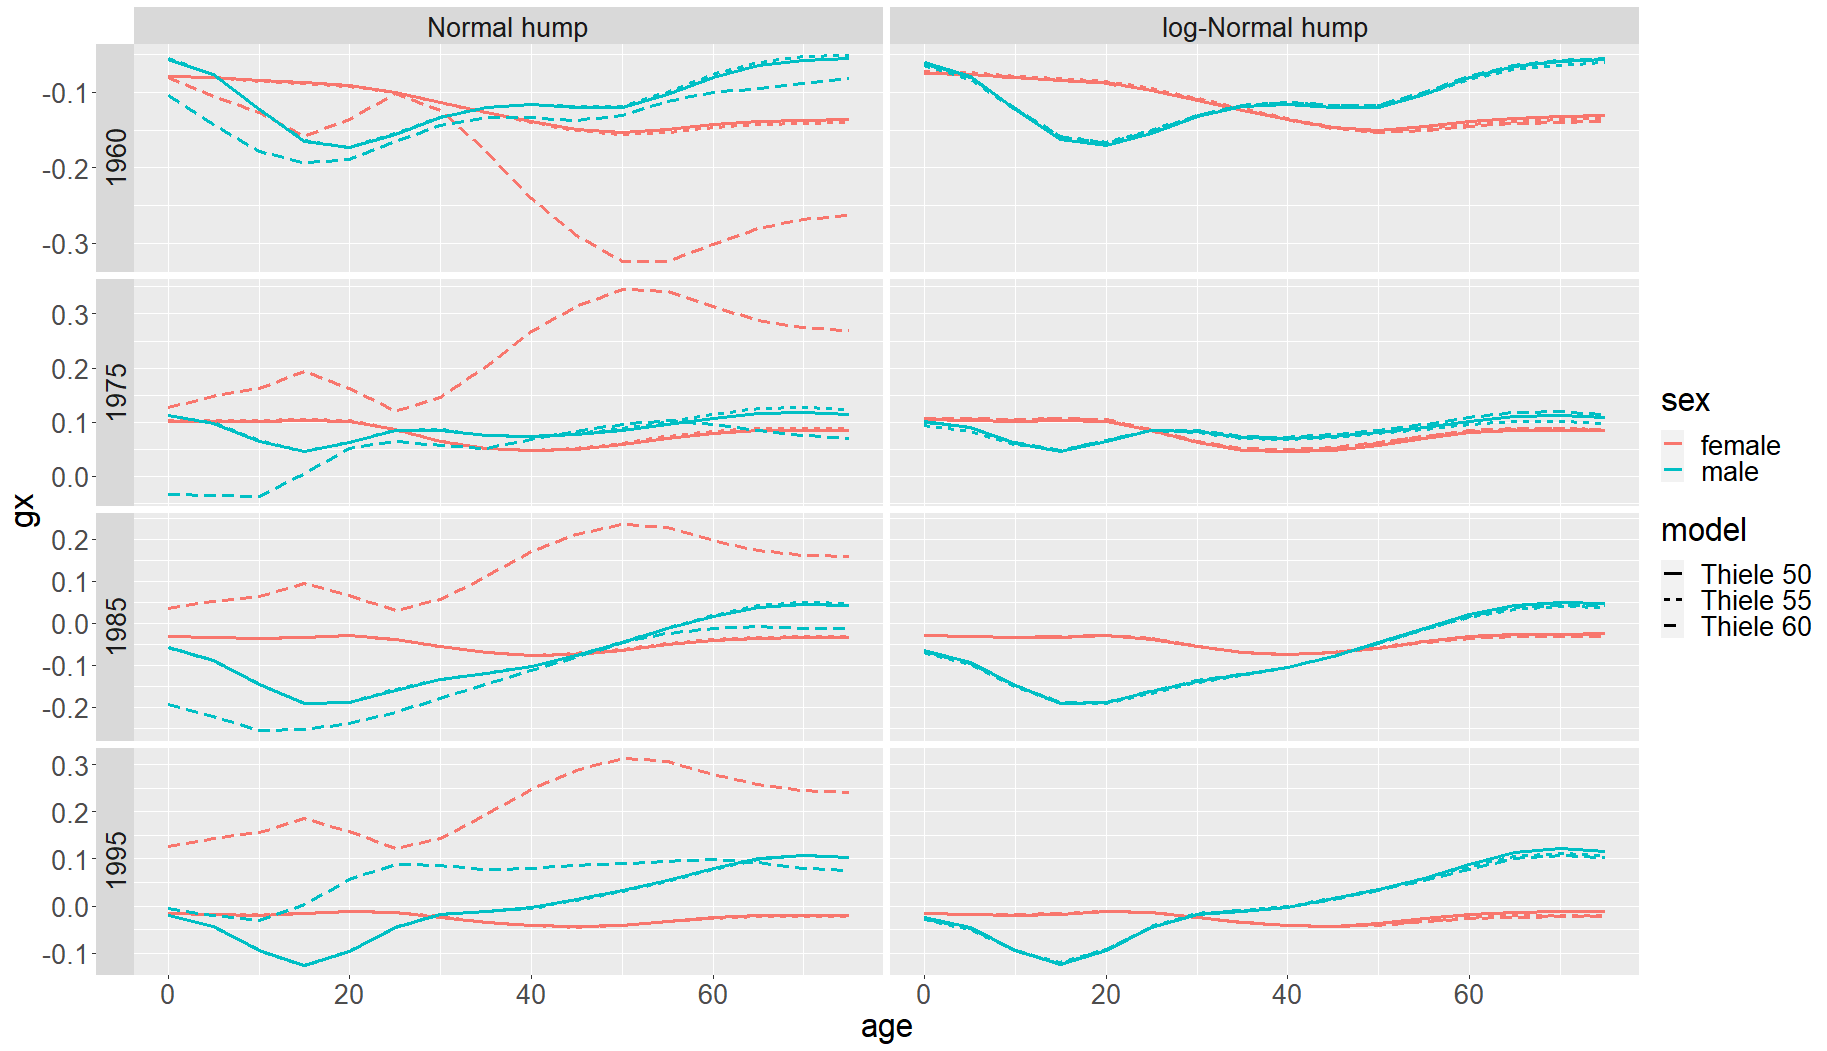
\includegraphics[width = \linewidth]{mig.png}
\end{figure}
\begin{figure}[H]
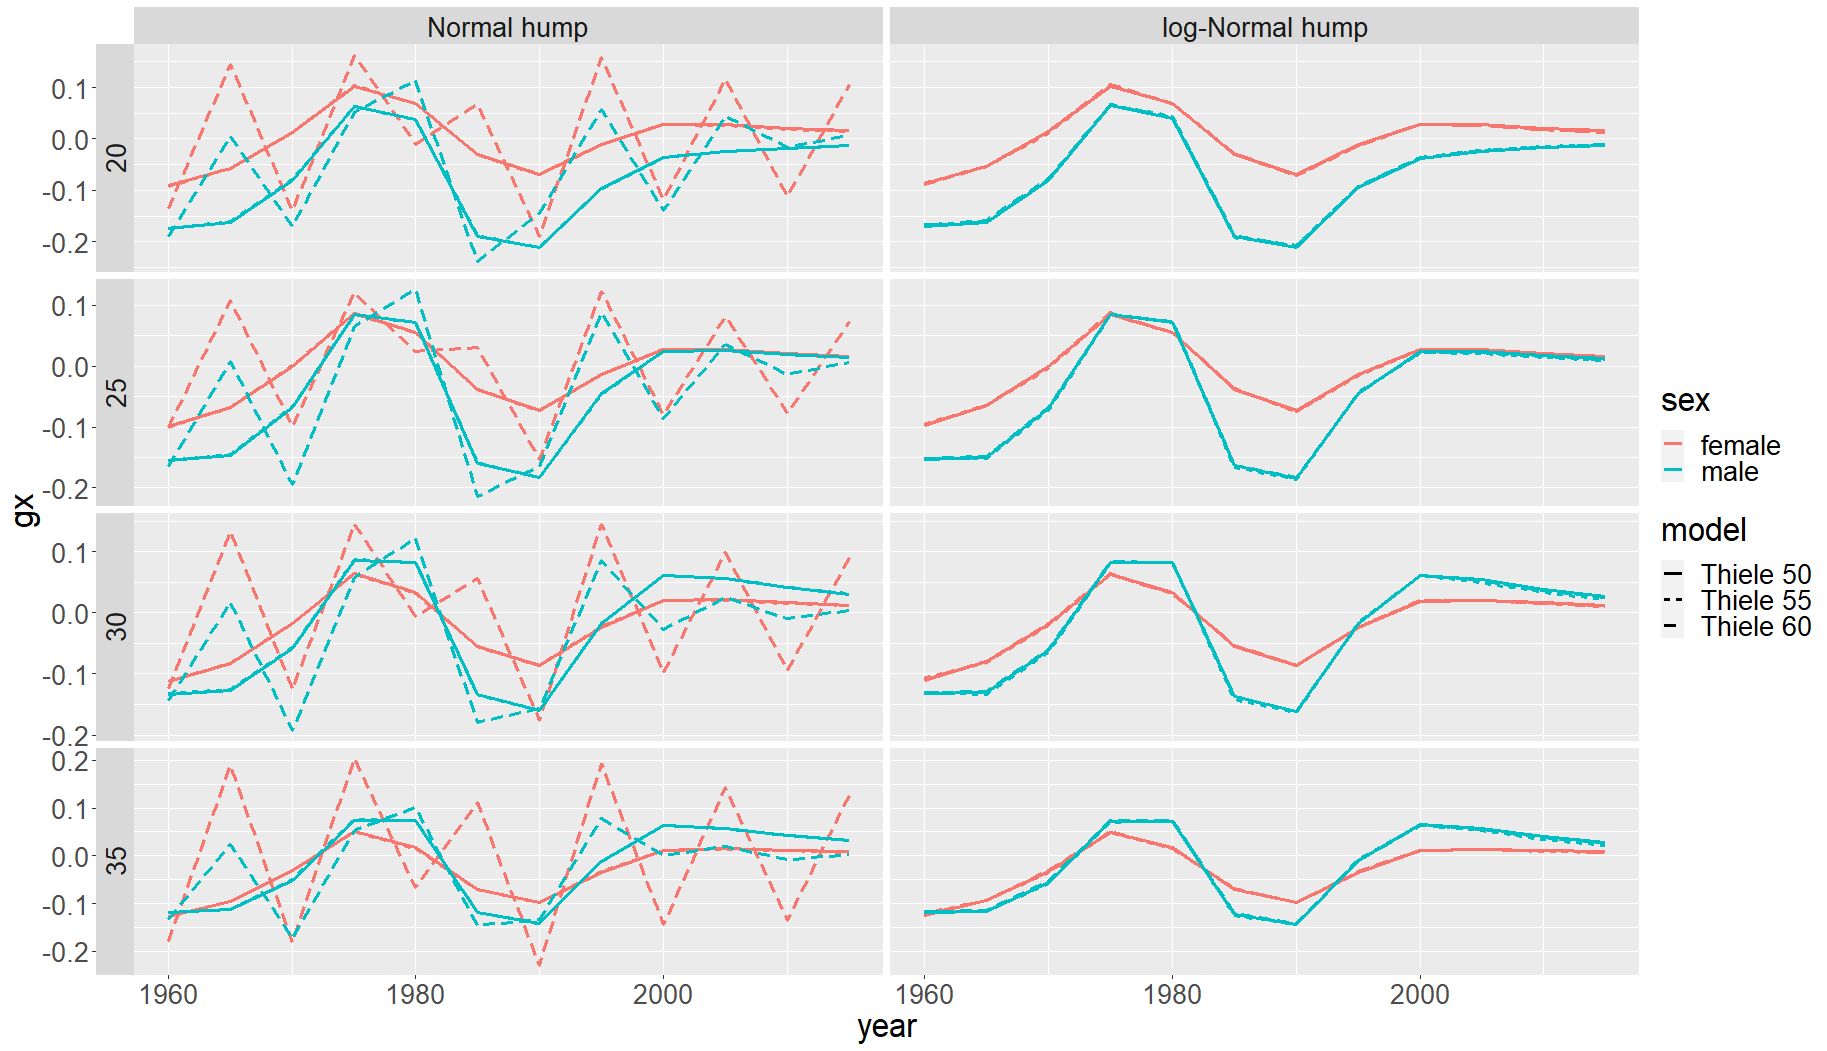
\includegraphics[width = \linewidth]{age mig.png}
\end{figure}

\newpage
\begin{figure}[H]
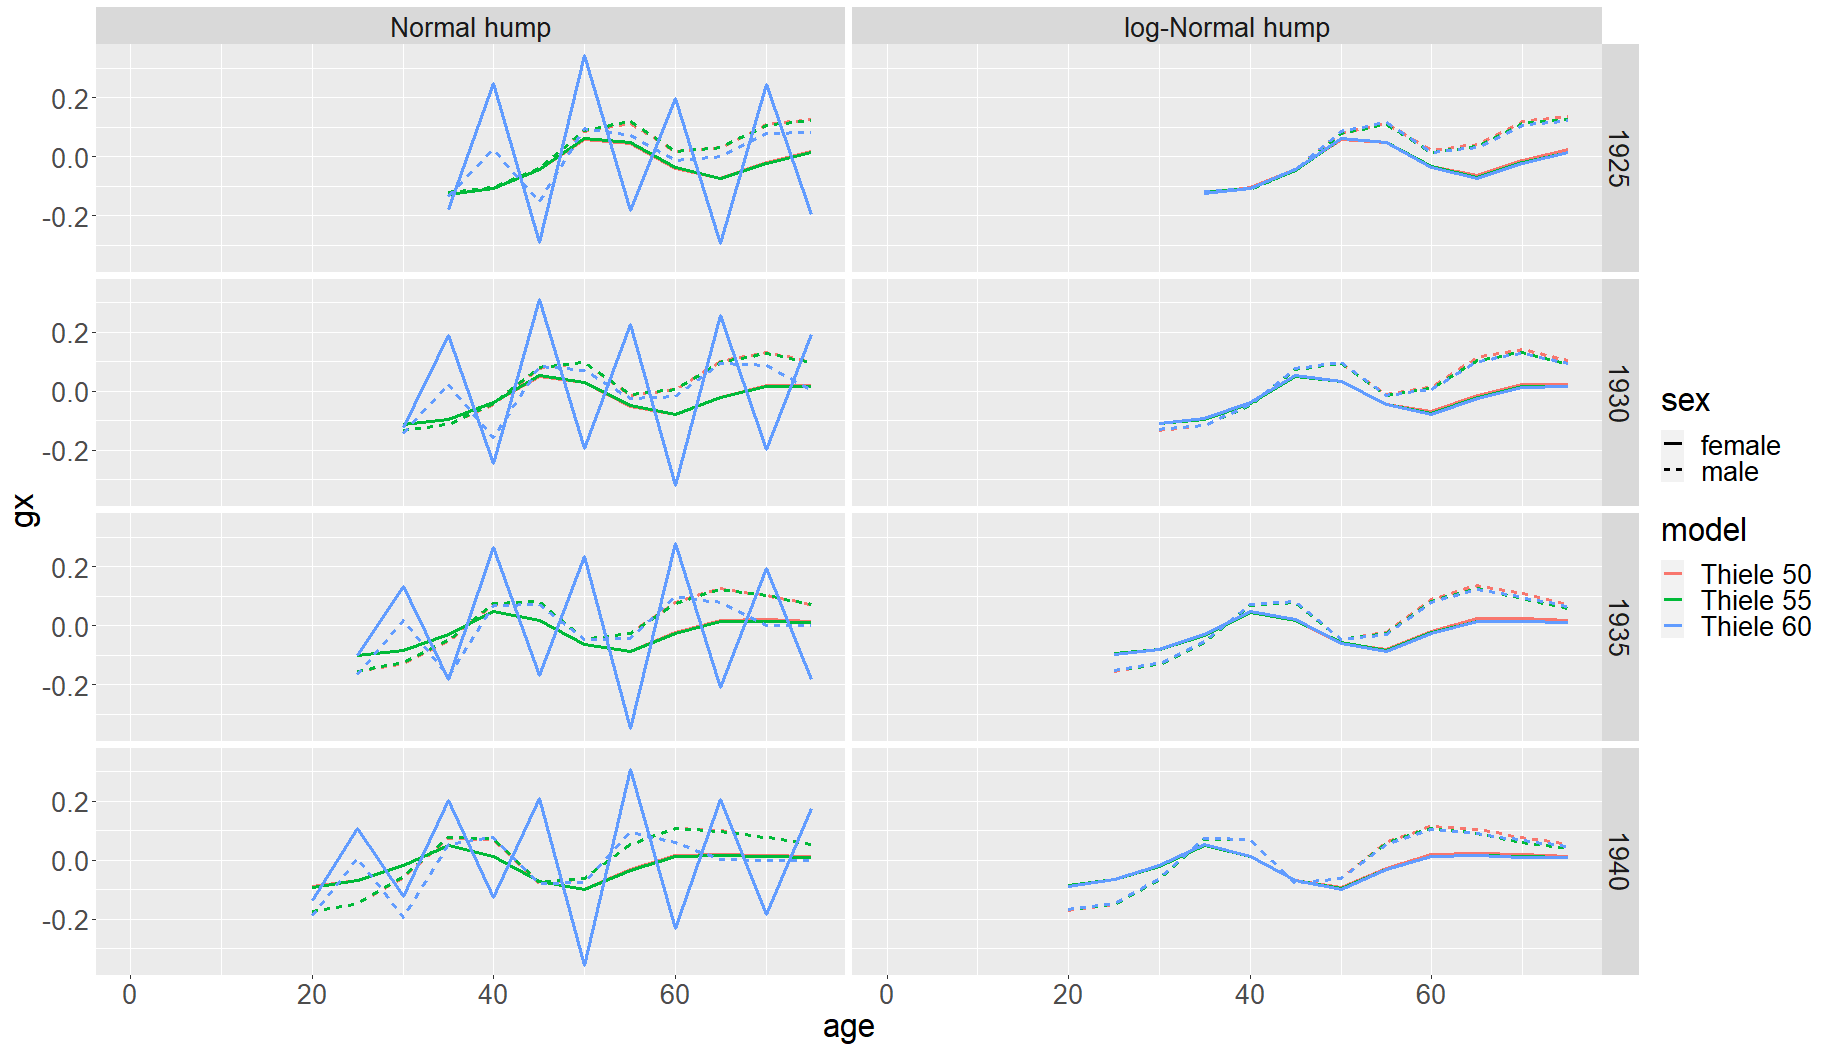
\includegraphics[width = \linewidth]{cohort mig.png}
\end{figure}

\newpage
\begin{figure}[H]
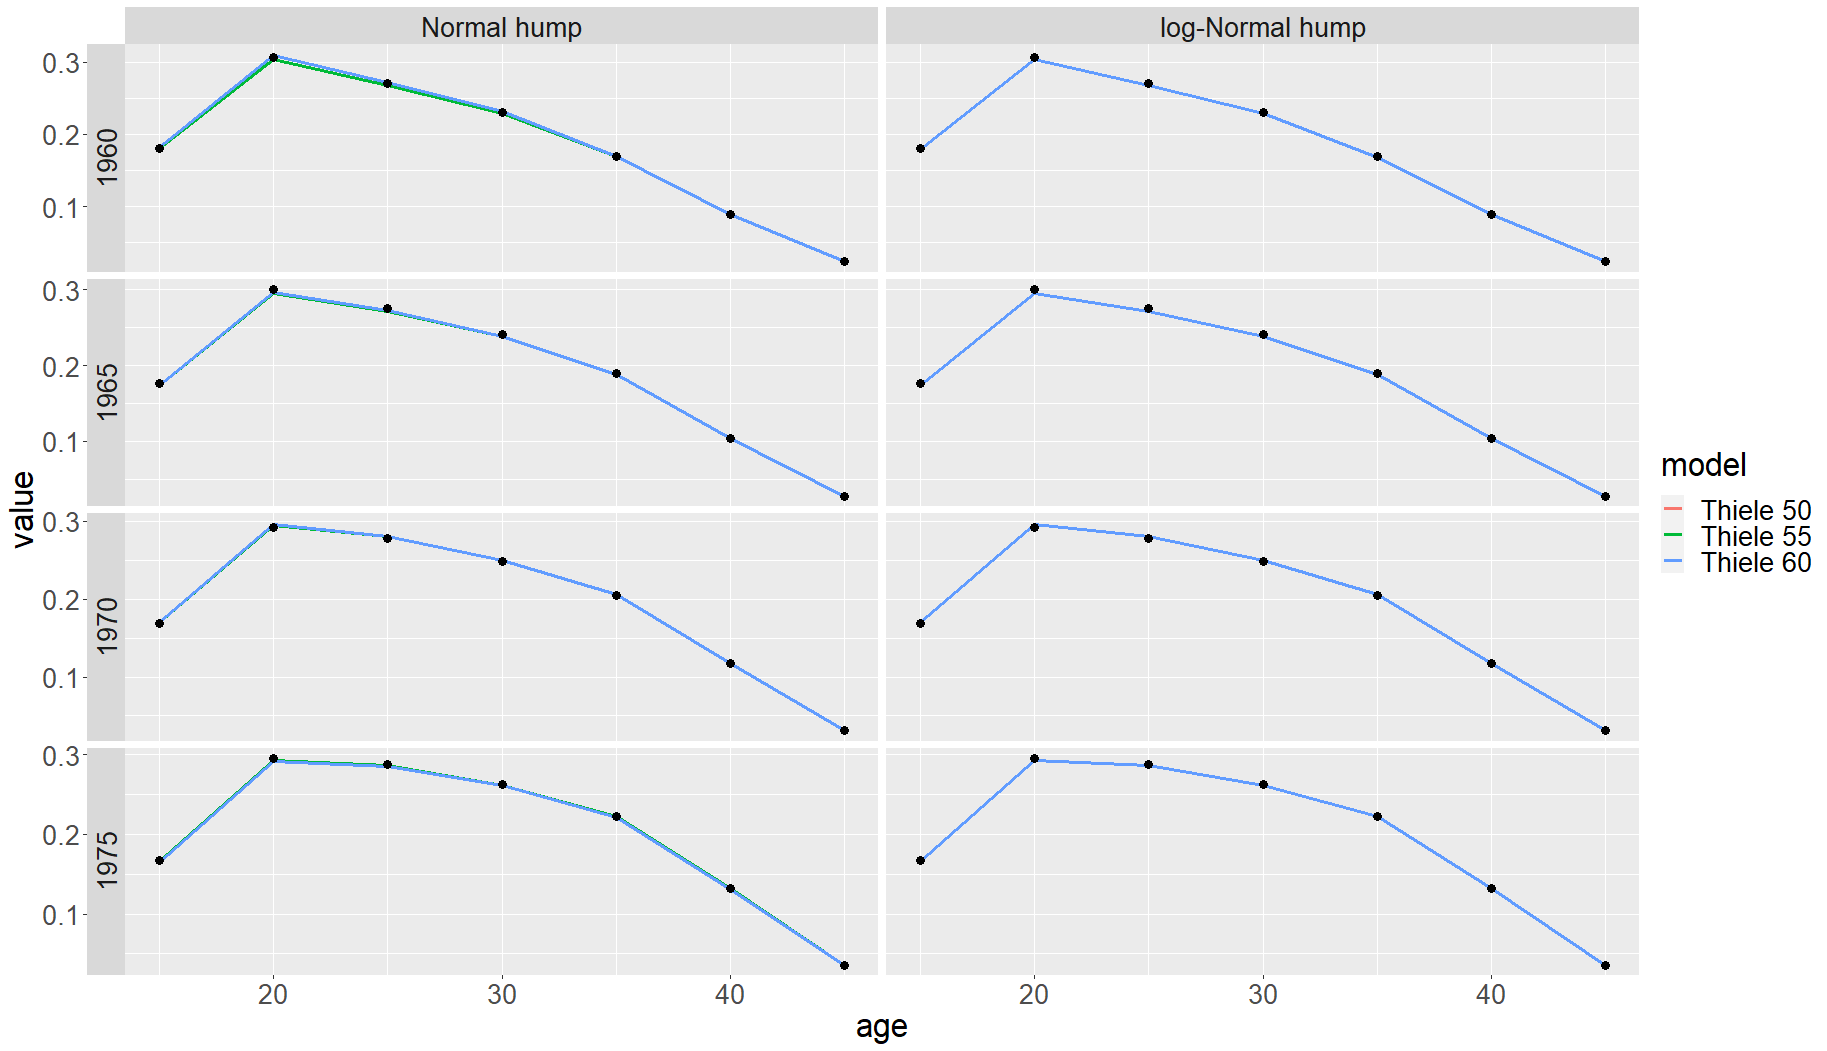
\includegraphics[width = \linewidth]{fert.png}
\end{figure}
\begin{figure}[H]
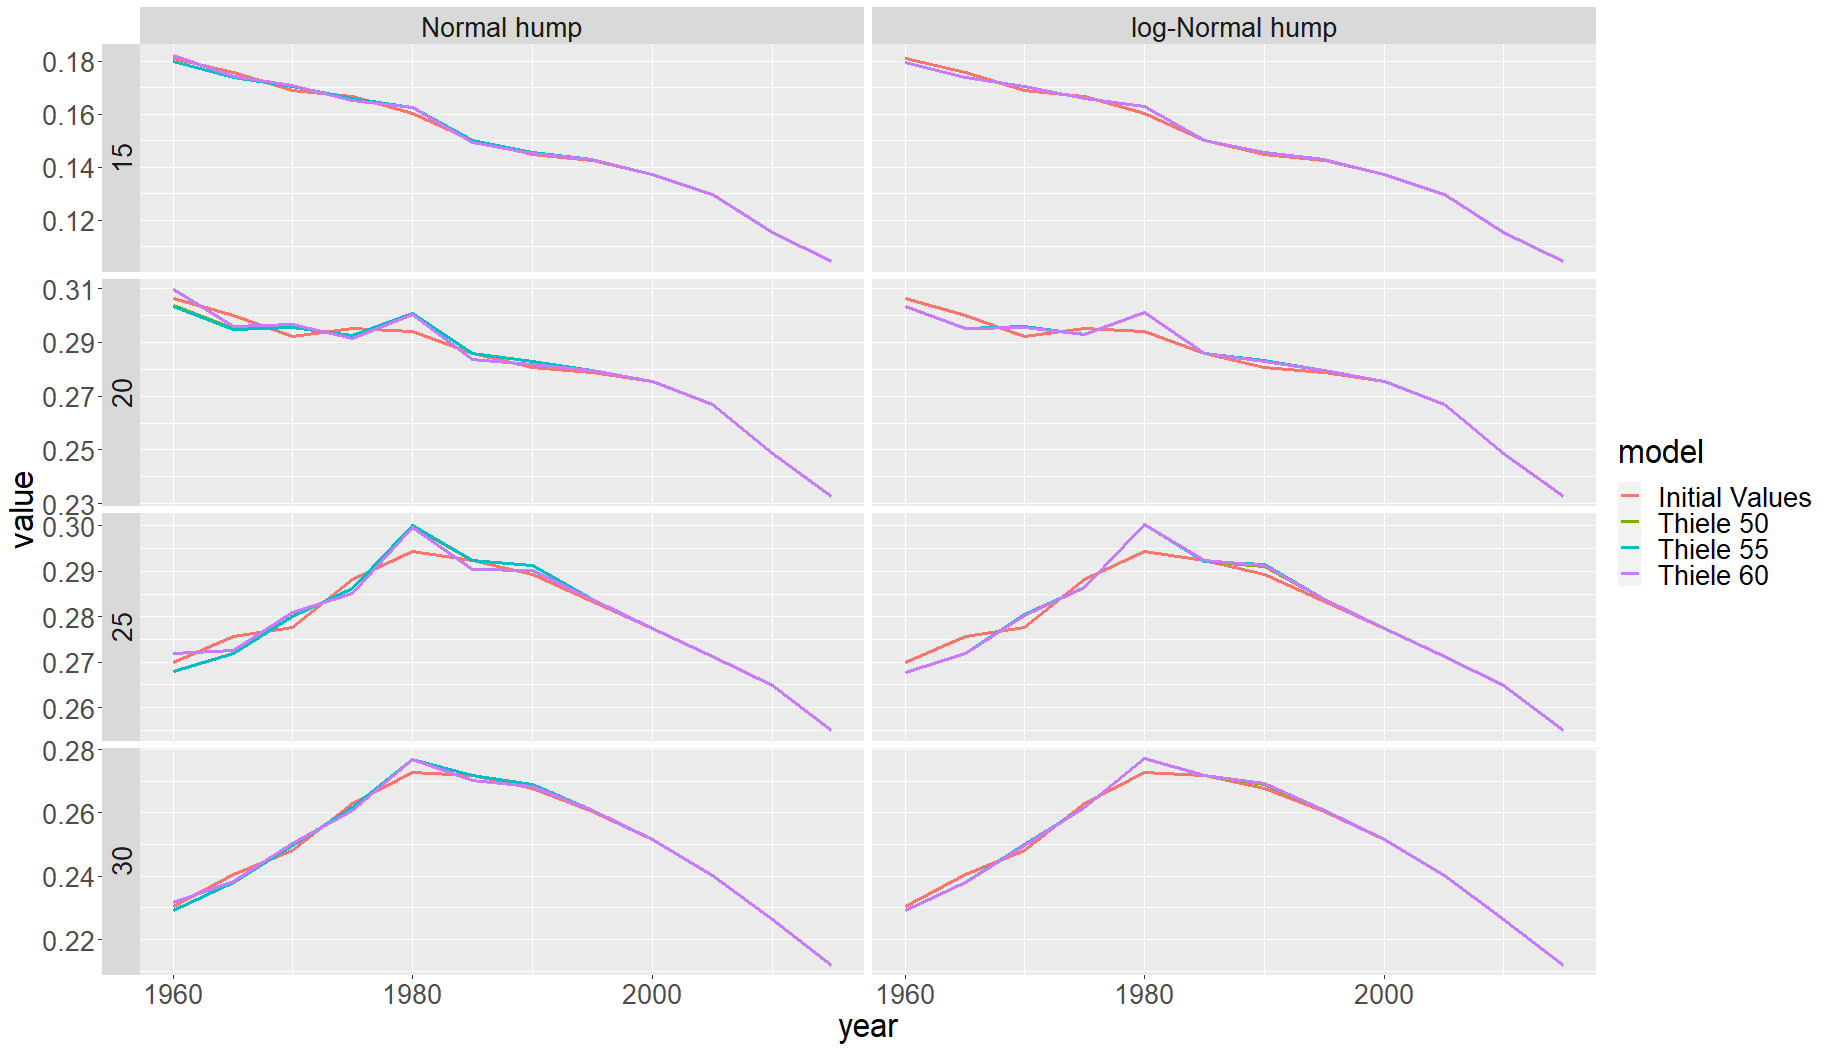
\includegraphics[width = \linewidth]{age fert.png}
\end{figure}


\newpage
\begin{figure}[H]
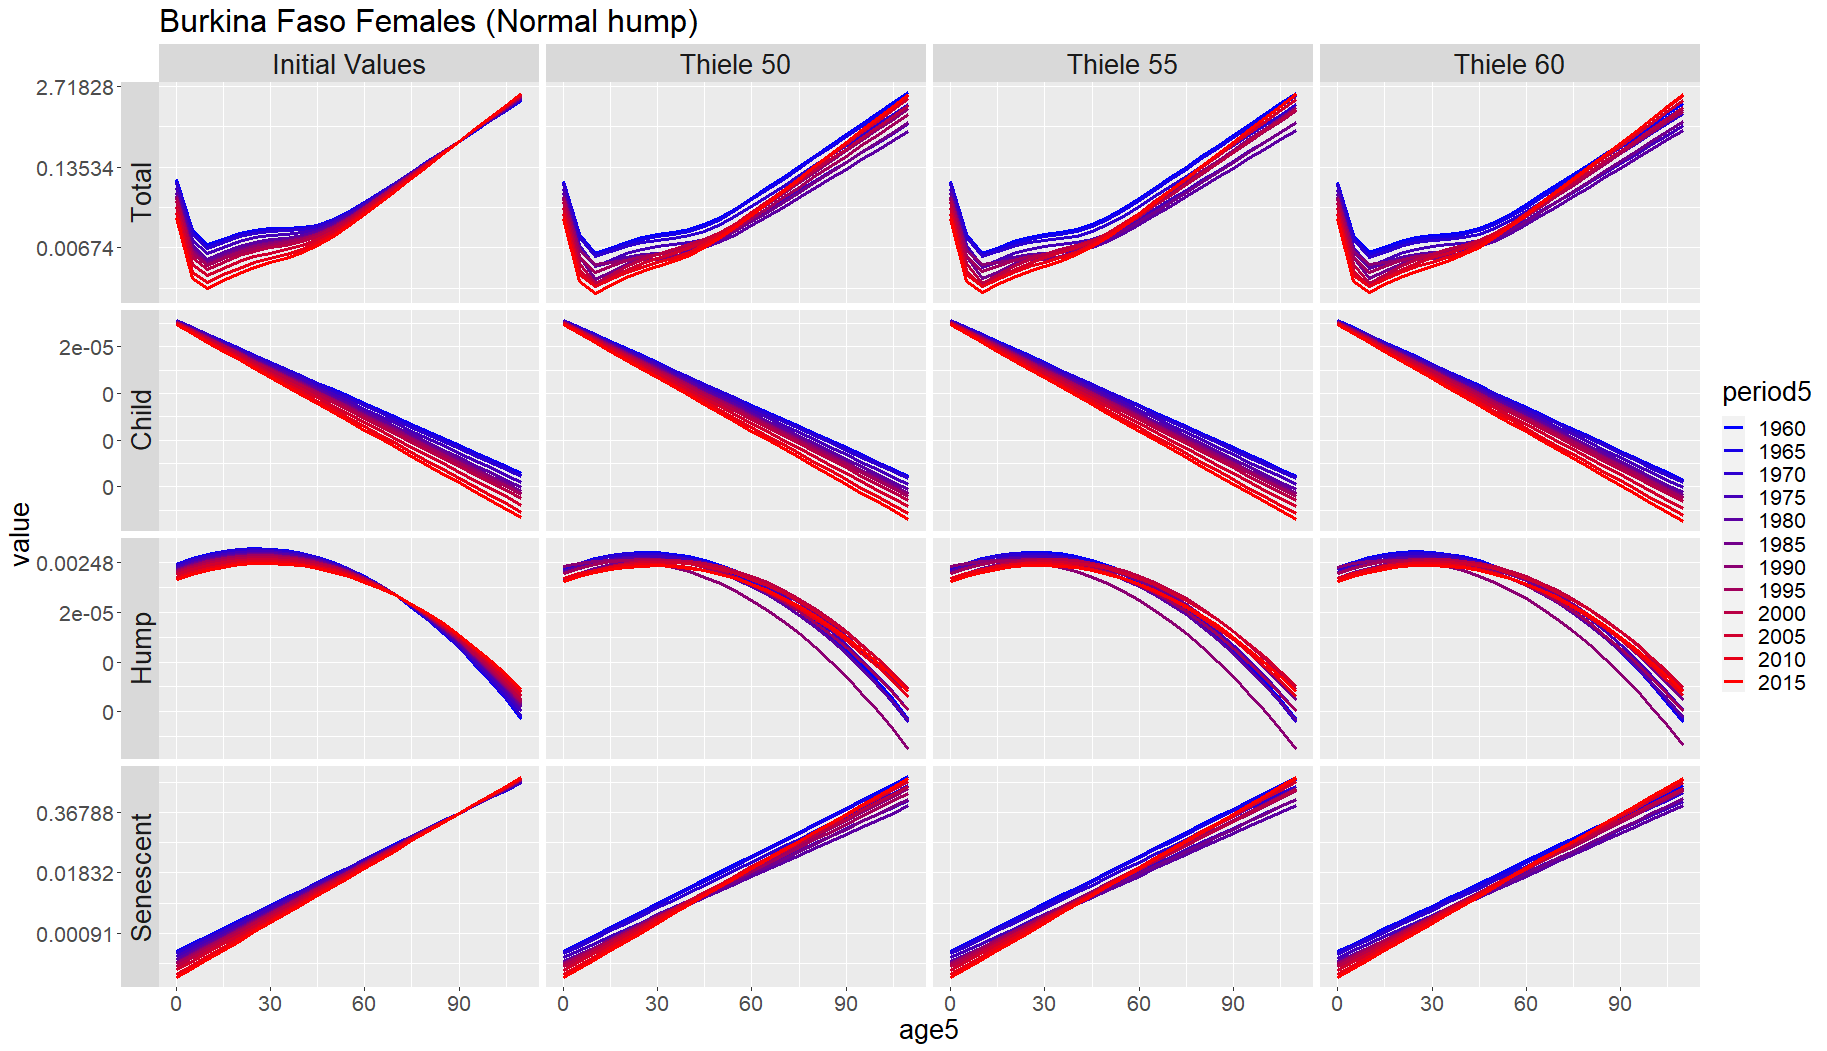
\includegraphics[width = \linewidth]{decomp females normal.png}
\end{figure}
\begin{figure}[H]
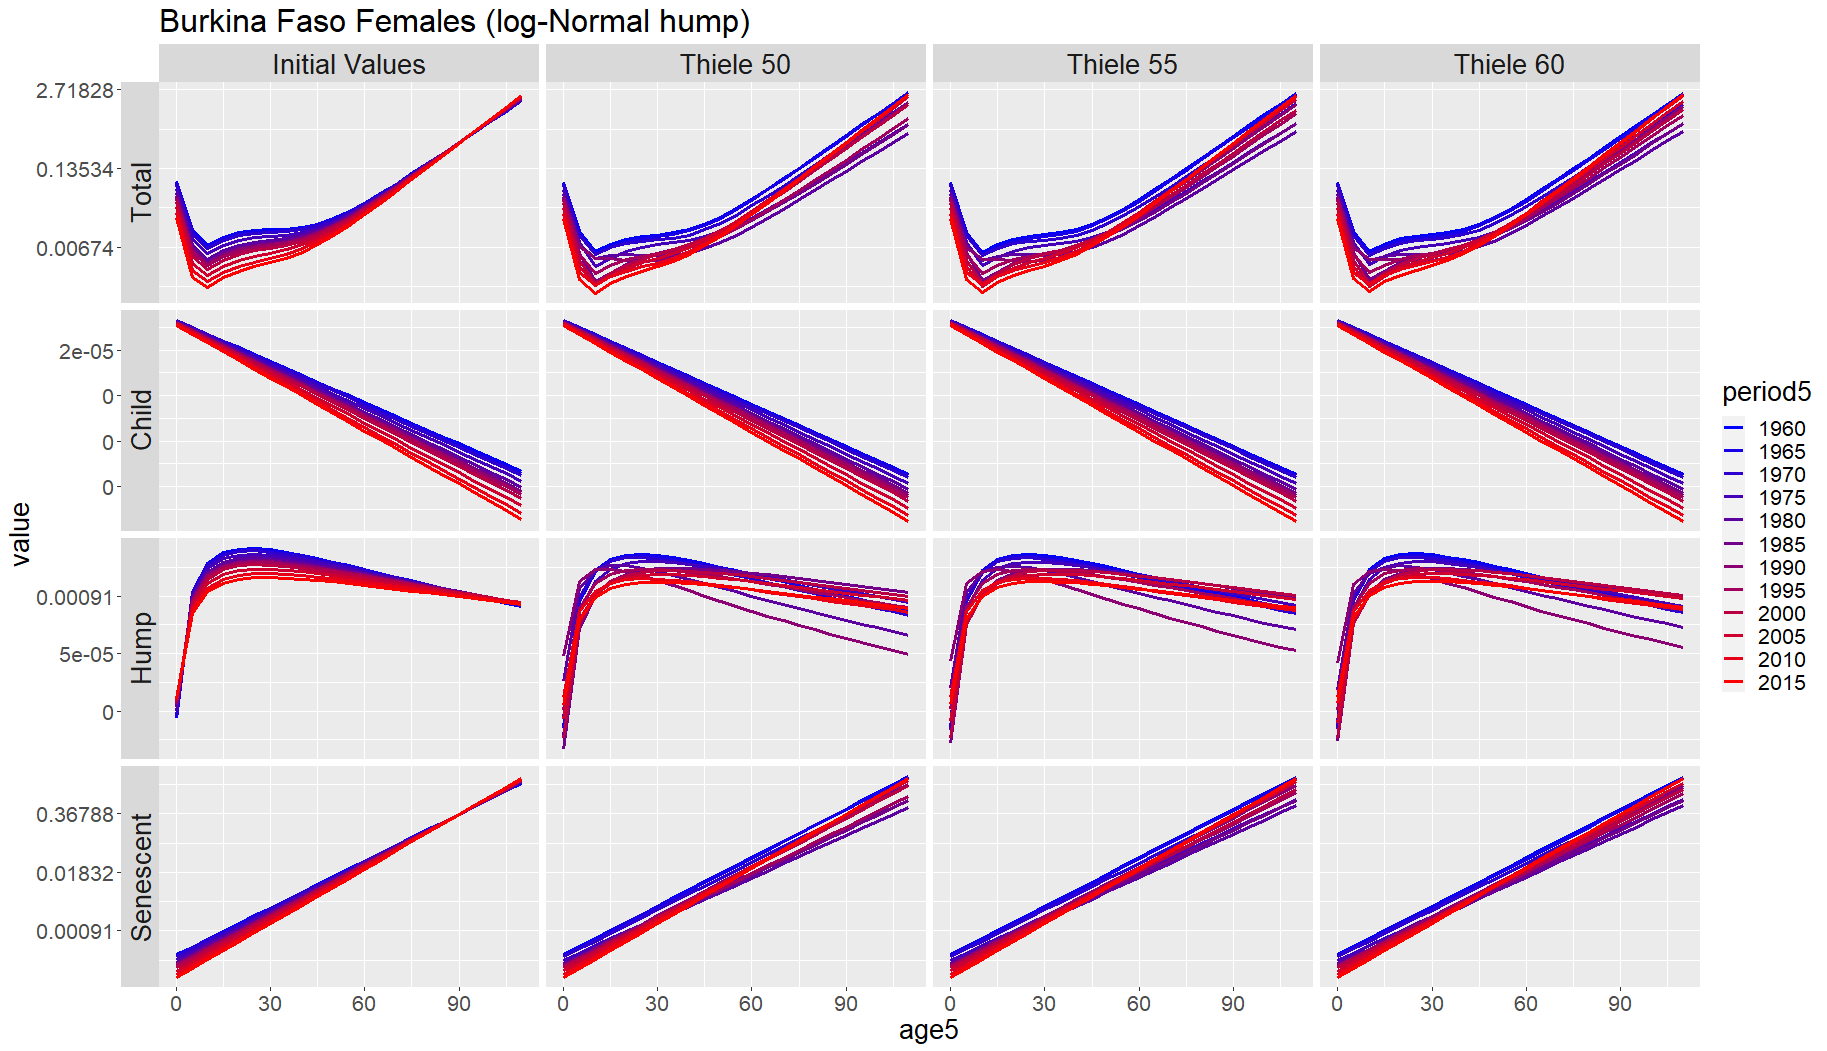
\includegraphics[width = \linewidth]{decomp females log-normal.png}
\end{figure}

\newpage
\begin{figure}[H]
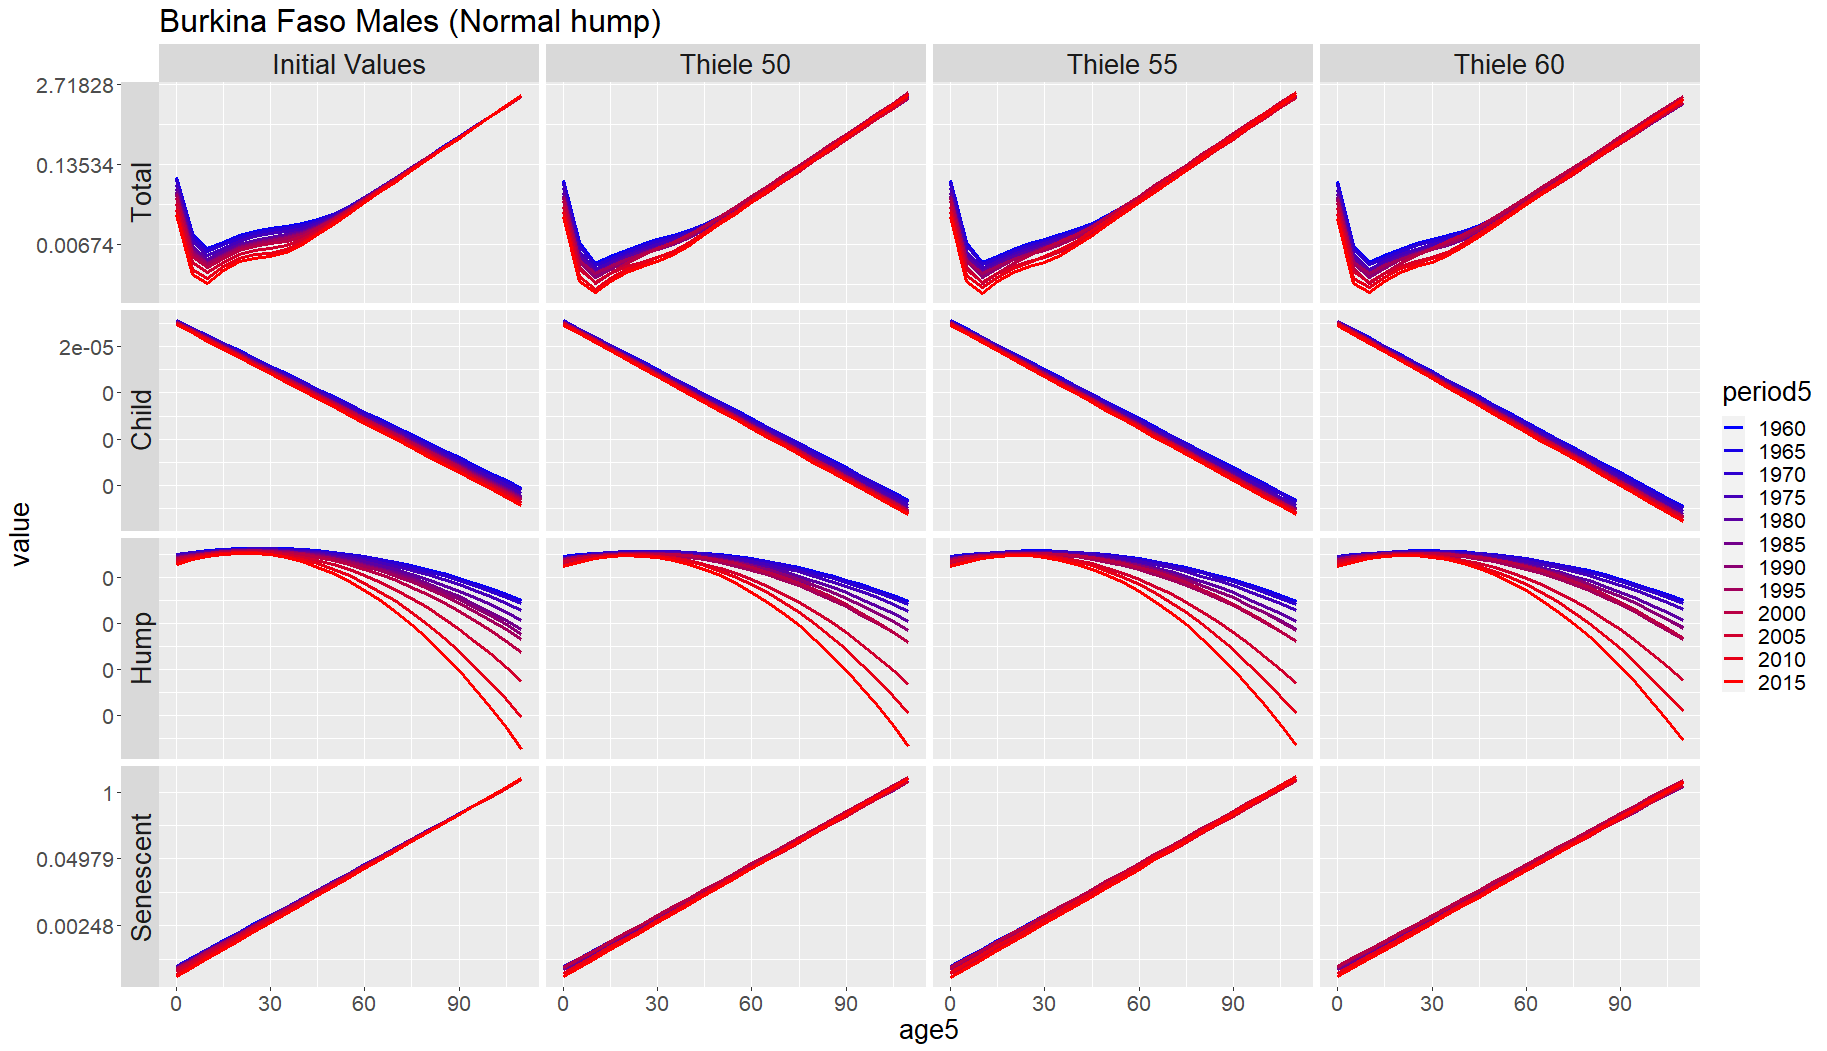
\includegraphics[width = \linewidth]{decomp males normal.png}
\end{figure}
\begin{figure}[H]
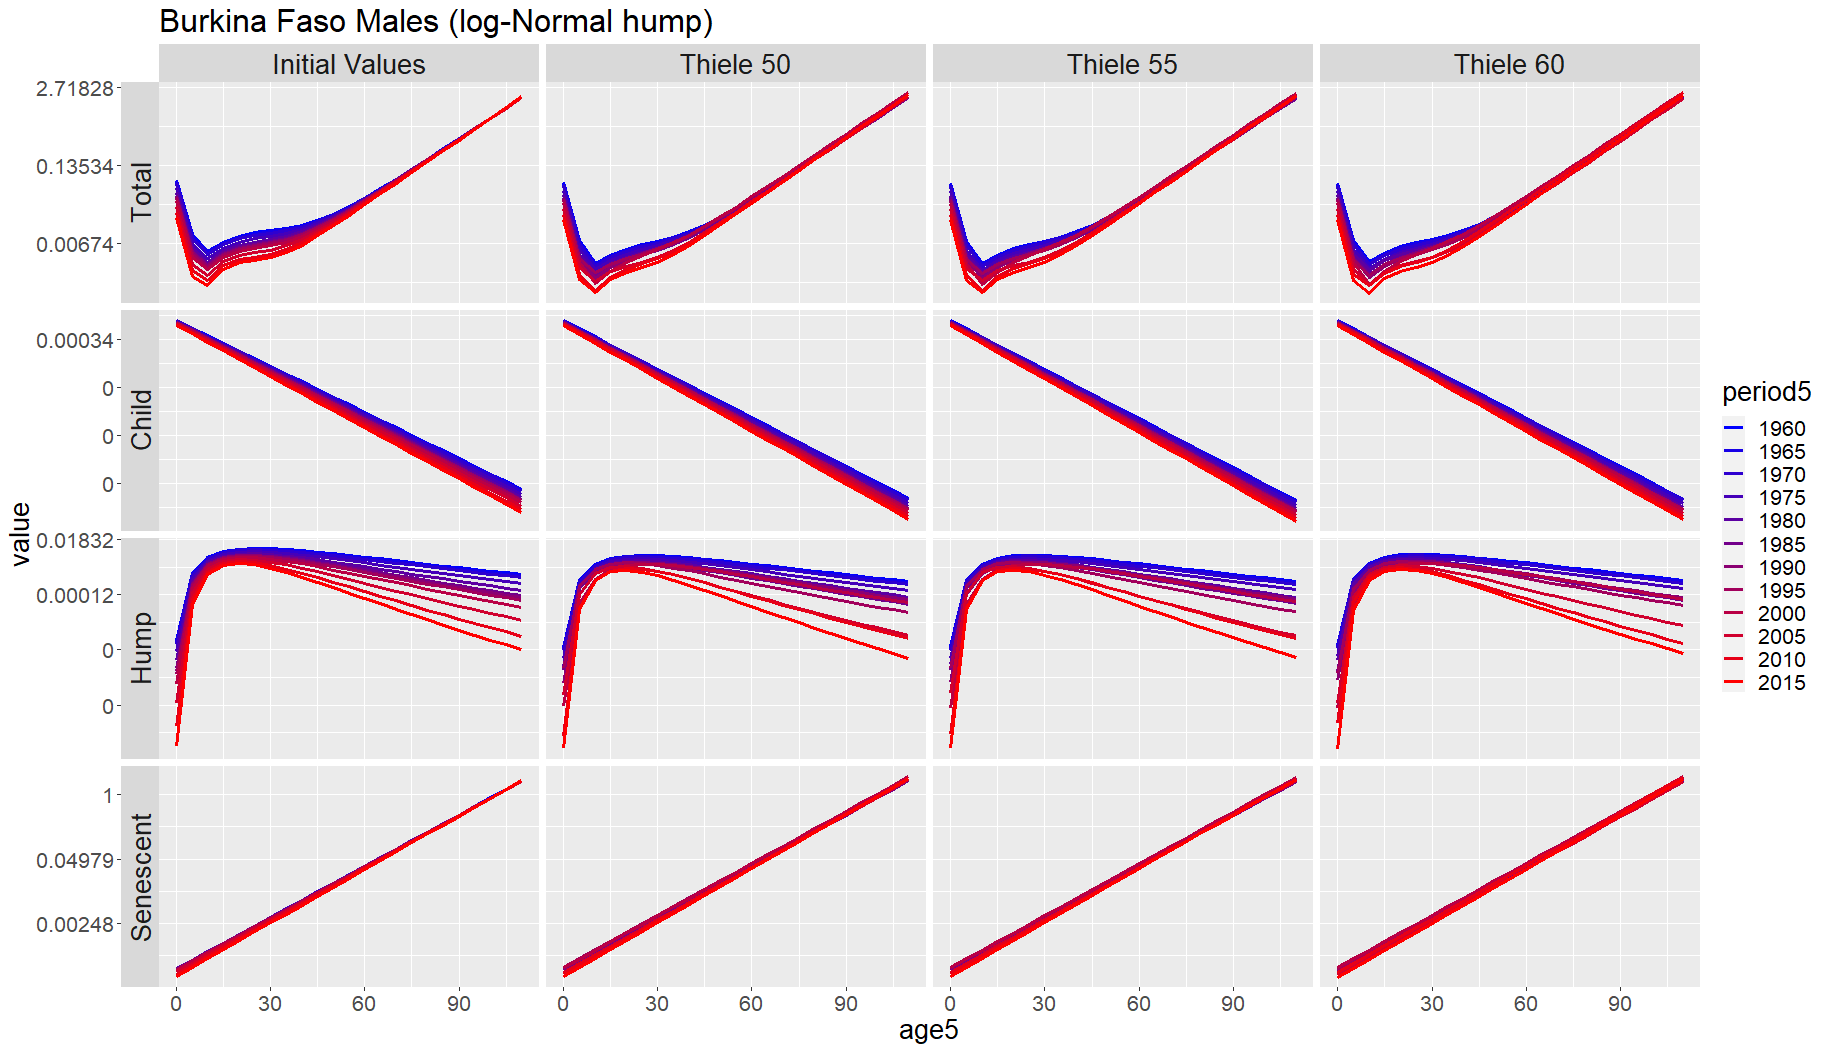
\includegraphics[width = \linewidth]{decomp males log-normal.png}
\end{figure}
\end{document} 